\documentclass[10pt]{article}
%\documentclass[10pt]{book}

\usepackage[draft]{fixme}

\usepackage{listings}
\usepackage{html}
\usepackage{color}
\usepackage{multicol}
\usepackage{multirow}
\usepackage{graphicx}
\usepackage{alltt}
% style for code listing
\lstset{language={C},basicstyle=\scriptsize} 
\newcommand{\hlstd}[1]{\textcolor[rgb]{0,0,0}{#1}}
\newcommand{\hlkey}[1]{\textcolor[rgb]{0,0,0}{\bf{#1}}}
\newcommand{\hlnum}[1]{\textcolor[rgb]{0.16,0.16,1}{#1}}
\newcommand{\hltyp}[1]{\textcolor[rgb]{0.51,0,0}{#1}}
\newcommand{\hlesc}[1]{\textcolor[rgb]{1,0,1}{#1}}
\newcommand{\hlstr}[1]{\textcolor[rgb]{1,0,0}{#1}}
\newcommand{\hldstr}[1]{\textcolor[rgb]{0.51,0.51,0}{#1}}
\newcommand{\hlcom}[1]{\textcolor[rgb]{0.51,0.51,0.51}{\it{#1}}}
\newcommand{\hldir}[1]{\textcolor[rgb]{0,0.51,0}{#1}}
\newcommand{\hlsym}[1]{\textcolor[rgb]{0,0,0}{#1}}
\newcommand{\hlline}[1]{\textcolor[rgb]{0.33,0.33,0.33}{#1}}

\newcommand{\mySmallFontSize}{\scriptsize}
\newcommand{\mySmallestFontSize}{\tiny}

\newcommand{\codeFontSize}{\scriptsize}
\newcommand{\code}[1]{{\scriptsize #1}}

% Software version number
%\newcommand{\VersionNumber}{@VERSION@}

%\newcommand{\ExampleDirectory}{@top_srcdir@/projects/compass/tests}

% Latex trick to allow us to comment out large sections of documentation
\newcommand{\commentout}[1]{}

% change the title of the Fixme List
\renewcommand{\listfixmename}{Things to Fix in Documentation}

\newcommand{\comm}[2]{\bigskip
                      \begin{tabular}{|p{11cm}|}\hline
                      \multicolumn{1}{|c|}{{\bf Comment by #1}}\\ \hline
                      #2\\ \hline
                      \end{tabular}
                      \bigskip
                     }

\def\verbatimfile#1{\begingroup
                    \@verbatim \frenchspacing \@vobeyspaces
                    \input#1 \endgroup
}

\newcounter{lineno}

% Taken from verbatimfiles.sty on web
\makeatletter %JCL

\def\verbatimlisting#1{\setcounter{lineno}{0}%
    \begingroup \@verbatim \frenchspacing \@vobeyspaces \parindent=20pt
    \everypar{\stepcounter{lineno}\llap{\thelineno\ \ }}\input#1
    \endgroup
}

\makeatother %JCL

% \endinput

\addtolength{\textheight}{0.5in}
\sloppy

%---------------------------------------------------------------------
% Begin Document
%---------------------------------------------------------------------

\begin{document}

% This draft mode eliminates the figures (leaves boxes for where they would be)
%\textcolor{green}{(Associated with ROSE Version @VERSION@)} } }
%\psdraft

\title{ {\bf \textcolor{red}{ROSE-Based End-to-End Empirical Tuning:} \\ 
              \textcolor{blue}{Draft User Tutorial} \\
%              \textcolor{green}{(Associated with ROSE Version @VERSION@)} 
              } }
\author{ {\bf Chunhua Liao and Dan Quinlan} \\
         Lawrence Livermore National Laboratory \\ 
         Livermore, CA  94550 \\
         925-423-2668 (office)  925-422-6278 (fax) \\
         {liao6, dquinlan}@llnl.gov \\
         Project Web Page:
         \htmladdnormallink{http://www.rosecompiler.org}{http://www.rosecompiler.org} \\
         UCRL Number for ROSE User Manual: UCRL-SM-210137-DRAFT \\
         UCRL Number for ROSE Tutorial: UCRL-SM-210032-DRAFT \\
         UCRL Number for ROSE Source Code: UCRL-CODE-155962 \\ \\
         \htmladdnormallink{ROSE User Manual
         (pdf)}{http://www.rosecompiler.org/ROSE_UserManual/ROSE-UserManual.pdf} \\
         \htmladdnormallink{ROSE Tutorial
         (pdf)}{http://www.rosecompiler.org/ROSE_Tutorial/ROSE-Tutorial.pdf} \\
         \htmladdnormallink{ROSE HTML Reference (html
         only)}{http://www.rosecompiler.org/ROSE_HTML_Reference/index.html}
       }
\maketitle
\newpage


% This fixes the really long table of contents problem
\setcounter{tocdepth}{1}

\tableofcontents
\newpage
%

\chapter{Introduction}

\section{Overview}

\label{introduction::overview}

   Compass is a tool for the checking of source code.  It is
based on the ROSE compiler infrastructure and demonstrates to
use of ROSE to build lots of simple pattern detectors for analysis
of C, C++, and Fortran source code.

   The purpose of this work is several fold:
\begin{itemize}
   \item Provide a concrete tool to support interactions with lab customers.
   \item Provide a home for the security analysis specific detectors being built within
         external research projects.
   \item Provide an external tool for general analysis of software.
   \item Provide a tool to support improvements to the ROSE source code base.
   \item Define an infrastructure for an evolving and easily tailored program analysis tool.
   \item Provide a simple motivation for expanded use of ROSE by external users.
         Development, testing, and evaluation of ROSE infrastructure is best facilitated 
         through its expanded use by others and this provides a specific and attractive
         tool that can provide feedback to users about their own code projects.  Even
         though optimization research is our focus, this gets our supporting
         infrastructure for optimization research out and into use by others in the form
         of an extensible tool.
\end{itemize}

   Note that as the collection of detectors grows we will periodically reorganize the 
collection.  At some point soon we will build a hierarchy to organize the evolving
collection.

%\subsection{A basis for other source analysis tools}
\paragraph{A basis for other source analysis tools}
   Input and output to ROSE is organized so that any number of source could be used.
So although we provide a compiler interface (for simplicity), we will also provide a 
GUI interface as an alternative interface to demonstrate that the detectors are orthogonal
to there use in alternative tools.  Alternative tool interfaces should be possible 
and will further demonstrate the independence of the input and output mechanisms to
the designs and implementation of the core detectors.

\paragraph{Add Your Own Detector}

    Detectors written in Compass make direct use of ROSE and are 
designed to be copied and extended by users to develop their own 
detectors. We welcome the contribution of these detectors back to 
the ROSE team for inclusion into future releases of Compass;
full credit for all work will be provide to all authors.
Compass is an open source project using ROSE, an open source
compiler infrastructure.

    Each of the detectors are examples of how to
add your own detector to {\bf Compass}.  If you
build a detector that you would like to have be 
distributed with {\bf Compass}, please send it to
us and we will add your as an external contributor.

  Guidelines for contributions:
\begin{itemize}
   \item Use any Compass detector and an example.
   \item provide the documentation about your detector.
   \item Use any features in ROSE to support your detector; AST, Control Flow graph,
    System dependence Graph, Call Graph, Class Hierarchy Graph, etc.
   \item Your detector should have {\bf NO} side-effects on the AST.
\end{itemize}






\chapter{Design}


\section{Use Cases}

\label{design::UseCase}

Figure~\ref{Compass_usecase} shows the use cases of \emph{Compass}.
Compass as a tool is used to analyze source code. The analysis is triggered by the user who
selects which detectors to execute. The user also specifies the source code to be checked.
Results of the analysis are presented to that user.

\begin{figure}[th]
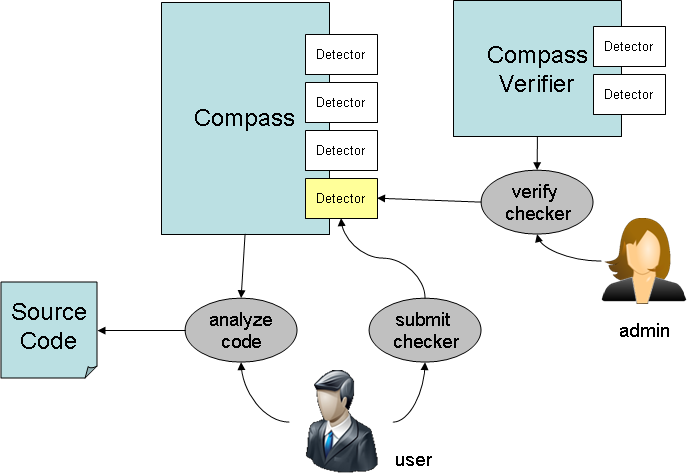
\includegraphics[width=4.5in]{compass_pic.png}
\caption{Compass Use Case}
\label{Compass_usecase}
\end{figure}

Furthermore, a user may contribute with his own detectors that he can add to Compass. Since 
external users may contribute detectors automatically via scripts, a verification of the 
validity and safety of these detectors is necessary. We provide a \emph{Compass Verifier}
that helps to check that all detectors are safe. Currently, the verifier is run by
a administrative person but may run automatically in the future.



\section{Design}

\begin{figure}[thb]
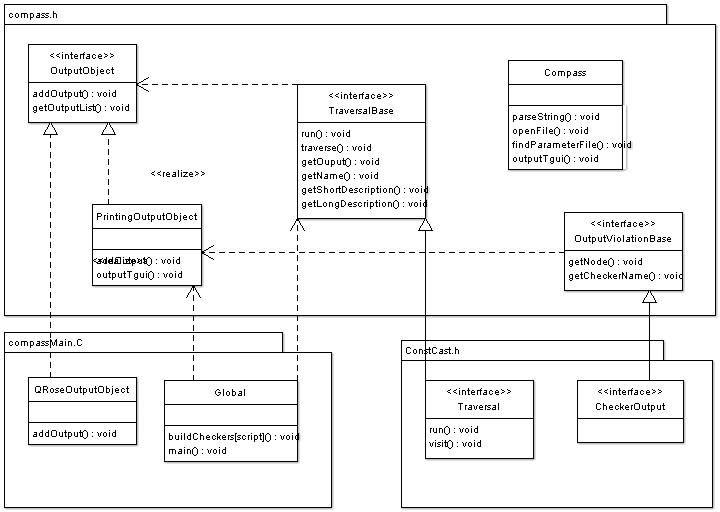
\includegraphics[width=6.0in]{compassdesign.png}
\caption{Compass Design}
\label{CompassDesign}
\end{figure}

Compass is designed to be easy to extend. Any user may write a detector and add it to Compass. Figure~\ref{CompassDesign}
illustrates the UML design decisions behind Compass.


Most of the functionality of Compass is in abstract classes hidden in the Compass namespace within compass.h - a file within
the compassSupport directory. All detectors, such as ConstCast illustrated in the figure, utilize the abstract classes
to traverse a program with all its nodes and to output violations found in that code according to the local algorithm.

CompassMain is the main executable that initially calls ROSE to parse a program. Then \emph{buildCheckers} is called to
load all detectors that are specified within a configuration file. The configuration file allows users to turn on and off
specific detectors for their run-time analyses. However, the configuration file only permits detectors to be loaded that 
were part of Compass at compile-time.

The main interface file compass.h contains the abstract classes \emph{TraversalBase} and 
\emph{OutputObject}. TraversalBase is the interface to ROSE, allowing a detector to traverse the ROSE AST (program) and hence
perform analysis on that AST. OutputObject aids to output defects found by a specific detector. More functionality to handle
e.g. file input and parameters provided to Compass, is provided within the Compass namespace.


\section{Compass Verifier}

\subsection{Threats} 

Compass must be safe, so that analyses and their results can be trusted. 
The main threats to the validity of Compass are:

\begin{itemize}
\item \emph{Malicious User}. A malicious user is an external user of Compass contributing a detector that performs malicious behaviour.  
\item \emph{Malicious Detector}. Compass is extensible and new detectos can be added externally (users outside the main development group).
  A detector can be programmed arbitrarily using the C/C++ and assembly programming languages. 
  It is therefore possible for a skilled programmer to hide malicious operations within a detector, e.g. allow a detector to scan the host machine and
  send data away. Compass must prevent detectors with malicious behaviour to be part of the Compass system. 
\item \emph{Source Code Replacement}. It should not be possible for users to exchange the source code of detectors within a running system,
  i.e. Compass cannot implement dynamic loading of detectors. Such a feature would compromise its safety.
\item \emph{Binary Replacement}. Another threat is the replacement of a valid Compass detector with a modified malicious version within a binary release of Compass.
  Therefore, Compass should be aware if parts of itself were modified and should not execute.
\end{itemize} 

\subsection{Safety Handling}

Compass is designed to be safe. The Compass Verifier is a stable separate copy of Compass that contains only a few detectors
to check (external and internal) user delivered detectors for safety. We have designed Compass in a way that it addresses the threats mentioned above:

\begin{itemize}
\item \emph{Malicious User}. Initially, we permit only trusted individuals to add new detectors to Compass. Once the verification process
  is matured, we will extend this policy to allow arbitrary users to contribute to Compass. 

\item \emph{Malicious Detector}. To prevent Compass to execute malicious code, the Compass Verifier executes its own detectors on
any user defined detector that is beeing considered to be added to Compass.
Currently, the Compass Verifier contains three detectors:

\begin{itemize}
\item \emph{fileReadOnlyAccess} ensures that a user defined detector perorms no write or execute operations on files. 
\item \emph{forbiddenFunctions} is a white list of function calls permitted in a detector. This list contains functions
that are trusted and hence considered unharmful when integrated to Compass.
\item \emph{noAsmStmtsOps} searches for assembly instructions in a detector and flags those as unsafe.
\end{itemize}

\item \emph{Source Code Replacement}. Detectors can only be added at compile time to Compass, not at run-time.
This means that detectors (meaning the source code) cannot be exchanged against unsafe versions at run-time. Furthermore, we allow only 
the Compass tool builder (admin) to build versions of Compass that must pass the Compass Verifier.

\item \emph{Binary Replacement}. Our goal is to perform a MD5 checksum on all the detectors part of the binary Compass distribution before
  Compass is executed. In this way Compass will not run if parts of it were modified.
\end{itemize} 


%The above list contains an important subset of detectors that enforce Compass detectors to be safe. 
%Additional detectors can easily be added to that list.
%In the future, a detector submitted to Compass, should go first through the automatic verifier, before it is either 
%added to Compass or denied.  



\clearpage
%\newpage
\section{Preparation}
The preparation phase provides basic information about a target application's performance
behaviors. 
Such information can be obtained by many performance tools.
Currently, we accept performance data generated by both HPCToolkit and GNU gprof.
%Currently, the ROSE-HPCToolKit interface is used to accept performance data generated by HPCToolkit and GNU gprof.
%The interface is used to annotate ROSE AST with performance metrics to
%facilitate building automated performance analysis tools. 
%Detailed information about ROSE-HPCToolKit can be found in Chapter 44 of
%the ROSE tutorial. 
%We only give information relevant to autotuning below.

\subsection{Using HPCToolkit}
%The HPCToolkit~\cite{hpctoolkit} is developed at the Rice University to get
%performance metrics of the target application. 
The HPCToolkit~\cite{hpctoolkit}, developed at the Rice University, is an open source profile-based
performance analysis tool sampling the executions of optimized applications. No code
instrumentation is needed to use HPCToolkit. But debugging information (by compiling with
the -g option if GCC is used) in the binary executables is needed for the tool to
associate performance metrics with source language constructs.

After installation, a typical session of using HPCToolkit is given below:
{\mySmallFontSize
\begin{verbatim}
% Prepare the executable with debugging information
gcc -g smg2000.c -o smg2000 

% Sample one or more events for the execution, use wall clock here
hpcrun -e WALLCLK -- ./smg2000 -n 120 120 120 -d 3

% Convert the profiling result into a XML format
hpcproftt -p -D /home/liao6/svnrepos/benchmarks/smg2000 ./smg2000 \
  smg2000.WALLCLK.tux268.llnl.gov.10676.0x0 > result.xml

\end{verbatim}
}

\fixme{TODO: update the text when the latest release of HPCToolkit works
on 32-bit platforms}

%A SMG2000~\cite{BrownSemicoarsening2000} (Semicoarsening Multigrid Solver) benchmark from the ASCI Purple
%benchmark suite is chosen to exemplify the use of this system.

Fig.~\ref{fig:hpctoolkitSmg2000} shows the profiling results of SMG2000
using HPCToolkit. 
A statement in a loop takes more than 46\% execution time, which makes the
loop dominant, most expensive loop of the entire program.
\begin{figure}[htbp]  
	\centering
		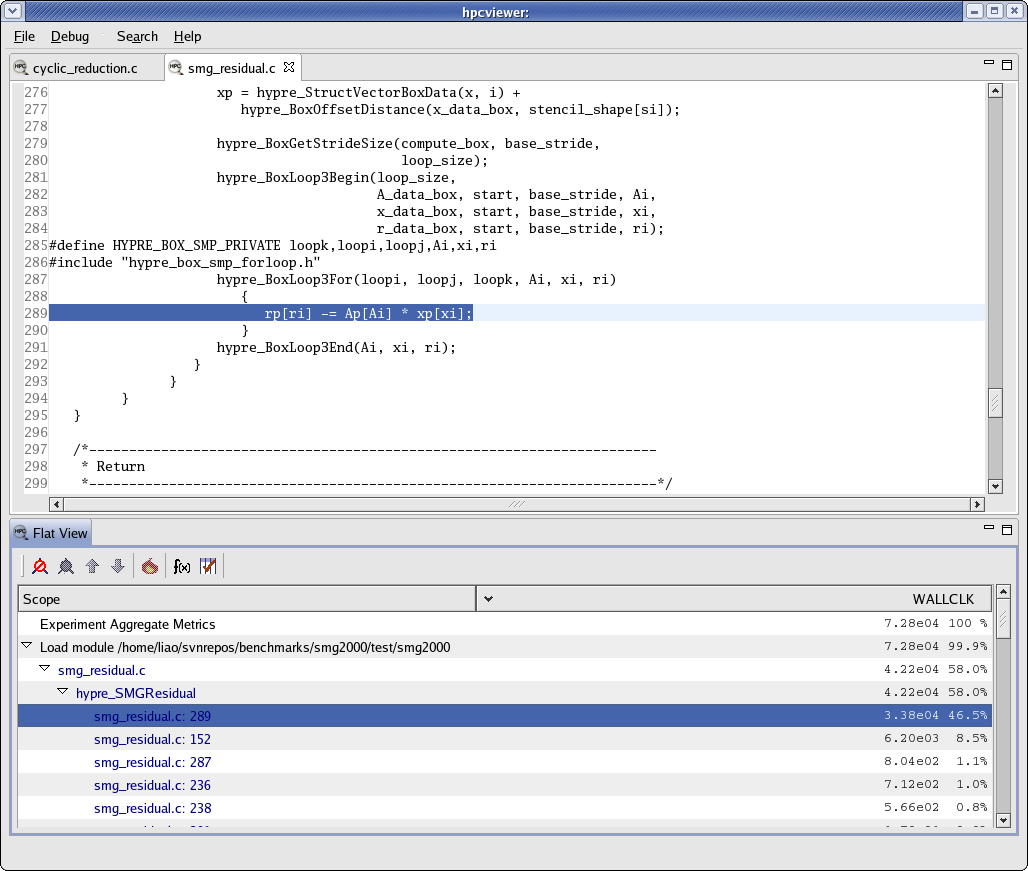
\includegraphics[width=0.9\textwidth]{hpctoolkit-smg2000.png}
	\caption{Profiling results of SMG2000 using HPCToolkit}
	\label{fig:hpctoolkitSmg2000}
\end{figure}

\subsection{Using gprof}
GNU gprof can generate line-by-line performance information for an
application. A typical session to generate such information is given below:
\begin{verbatim}
[liao@codes]$ gcc -g seq-pi.c -pg
[liao@codes]$ ./a.out
[liao@codes]$ gprof -l -L a.out gmon.out &>profile.result
\end{verbatim}

{\tt -l} tells gprof to output line-by-line profiling information and {\tt
-L} causes gprof to output full file path information. 

An excerpt of an output file for smg2000 looks like the following:
{\scriptsize
\begin{verbatim}
Flat profile:

Each sample counts as 0.01 seconds.
  %   cumulative   self     
 time   seconds   seconds     name
 35.01     13.08    13.08     hypre_SMGResidual (/home/liao/smg2000/struct_ls/smg_residual.c:289 @ 804caa4)
  9.05     16.46     3.38     hypre_CyclicReduction (/home/liao/smg2000/struct_ls/cyclic_reduction.c:1130 @ 8054af4)
  8.40     19.60     3.14     hypre_SMGResidual (/home/liao/benchmarks/smg2000/struct_ls/smg_residual.c:291 @ 804cab9)
  7.67     22.46     2.87     hypre_CyclicReduction (/home/liao/smg2000/struct_ls/cyclic_reduction.c:910 @ 8053191)
  5.97     24.70     2.23     hypre_CyclicReduction (/home/liao/smg2000/struct_ls/cyclic_reduction.c:998 @ 8053a28)
  5.27     26.66     1.97     hypre_SMGResidual (/home/liao/smg2000/struct_ls/smg_residual.c:238 @ 804d129)
  2.86     27.73     1.07     hypre_SMGResidual (/home/liao/smg2000/struct_ls/smg_residual.c:287 @ 804cacb)
  2.28     28.59     0.85     hypre_CyclicReduction (/home/liaosmg2000/struct_ls/cyclic_reduction.c:853 @ 8052bae)
  2.07     29.36     0.78     hypre_CyclicReduction (/home/liao/smg2000/struct_ls/cyclic_reduction.c:1061 @ 8054450)
  1.79     30.03     0.67     hypre_SemiRestrict (/home/liao/smg2000/struct_ls/semi_restrict.c:262 @ 8056a8c)
  1.67     30.66     0.62     hypre_SemiInterp (/home/liao/smg2000/struct_ls/semi_interp.c:294 @ 8055d6c)
  1.12     31.07     0.42     hypre_CyclicReduction (/home/liao/smg2000/struct_ls/cyclic_reduction.c:1133 @ 8054b2f)
  0.96     31.43     0.36     hypre_CyclicReduction (/home/liao/smg2000/struct_ls/cyclic_reduction.c:912 @ 80531a6)
  0.87     31.76     0.33     hypre_StructAxpy (/home/liao/smg2000/struct_mv/struct_axpy.c:69 @ 806642c)
  0.80     32.06     0.30     hypre_CyclicReduction (/home/liao/smg2000/struct_ls/cyclic_reduction.c:1002 @ 8053a60)
  0.78     32.35     0.29     hypre_SMGResidual (/home/liao/smg2000/struct_ls/smg_residual.c:236 @ 804d14b)
  0.72     32.62     0.27     hypre_CyclicReduction (/home/liao/smg2000/struct_ls/cyclic_reduction.c:1063 @ 8054462)
  0.60     32.84     0.23     hypre_SMGAxpy (/home/liao/smg2000/struct_ls/smg_axpy.c:69 @ 8064970)
  0.59     33.06     0.22     hypre_CycRedSetupCoarseOp (/home/liao/smg2000/struct_ls/cyclic_reduction.c:369 @ 8051149)
  0.59     33.28     0.22     hypre_SMGResidual (/home/liao/smg2000/struct_ls/smg_residual.c:240 @ 804d146)
  0.51     33.48     0.19     hypre_StructVectorSetConstantValues (/home/liao/smg2000/struct_mv/struct_vector.c:578 @ 806fedc)
  0.48     33.66     0.18     hypre_SMGSetupInterpOp (/home/liao/smg2000/struct_ls/smg_setup_interp.c:292 @ 804ea04)
  0.46     33.83     0.17     hypre_SemiInterp (/home/liao/smg2000/struct_ls/semi_interp.c:227 @ 80556e8)
  0.40     33.98     0.15     hypre_CyclicReduction (/home/liao/smg2000/struct_ls/cyclic_reduction.c:855 @ 8052bd4)
  0.40     34.12     0.15     hypre_StructMatrixInitializeData (/home/liao/smg2000/struct_mv/struct_matrix.c:359 @ 80678b0)
  ...
\end{verbatim}
}



%We use the self seconds associated with each source line and attach them to
%ROSE AST as AST attributes named WALLCLK.


\clearpage
\section{Code Triage and Transformations}
The second phase (shown in Fig.~\ref{fig:phase12}) includes code triage and a set of code transformations. 
Code triage relies on a ROSE-based tool interface to read in both source files and performance information of
the input application.
It then conducts various automated or user-directed analyses to identify
problematic code segments, such as loops. 
Finally, the identified code segments are extracted (also called outlined) into separated routines so they can be individually
optimized by empirical methods. 
%Since the analysis is on the AST or other graphs built
%using ROSE and uses the performance data stored as attributes, these analyses are
%expressed using traversals in ROSE.
\begin{figure}[htbp]
\vspace{5ex}
       \centering
               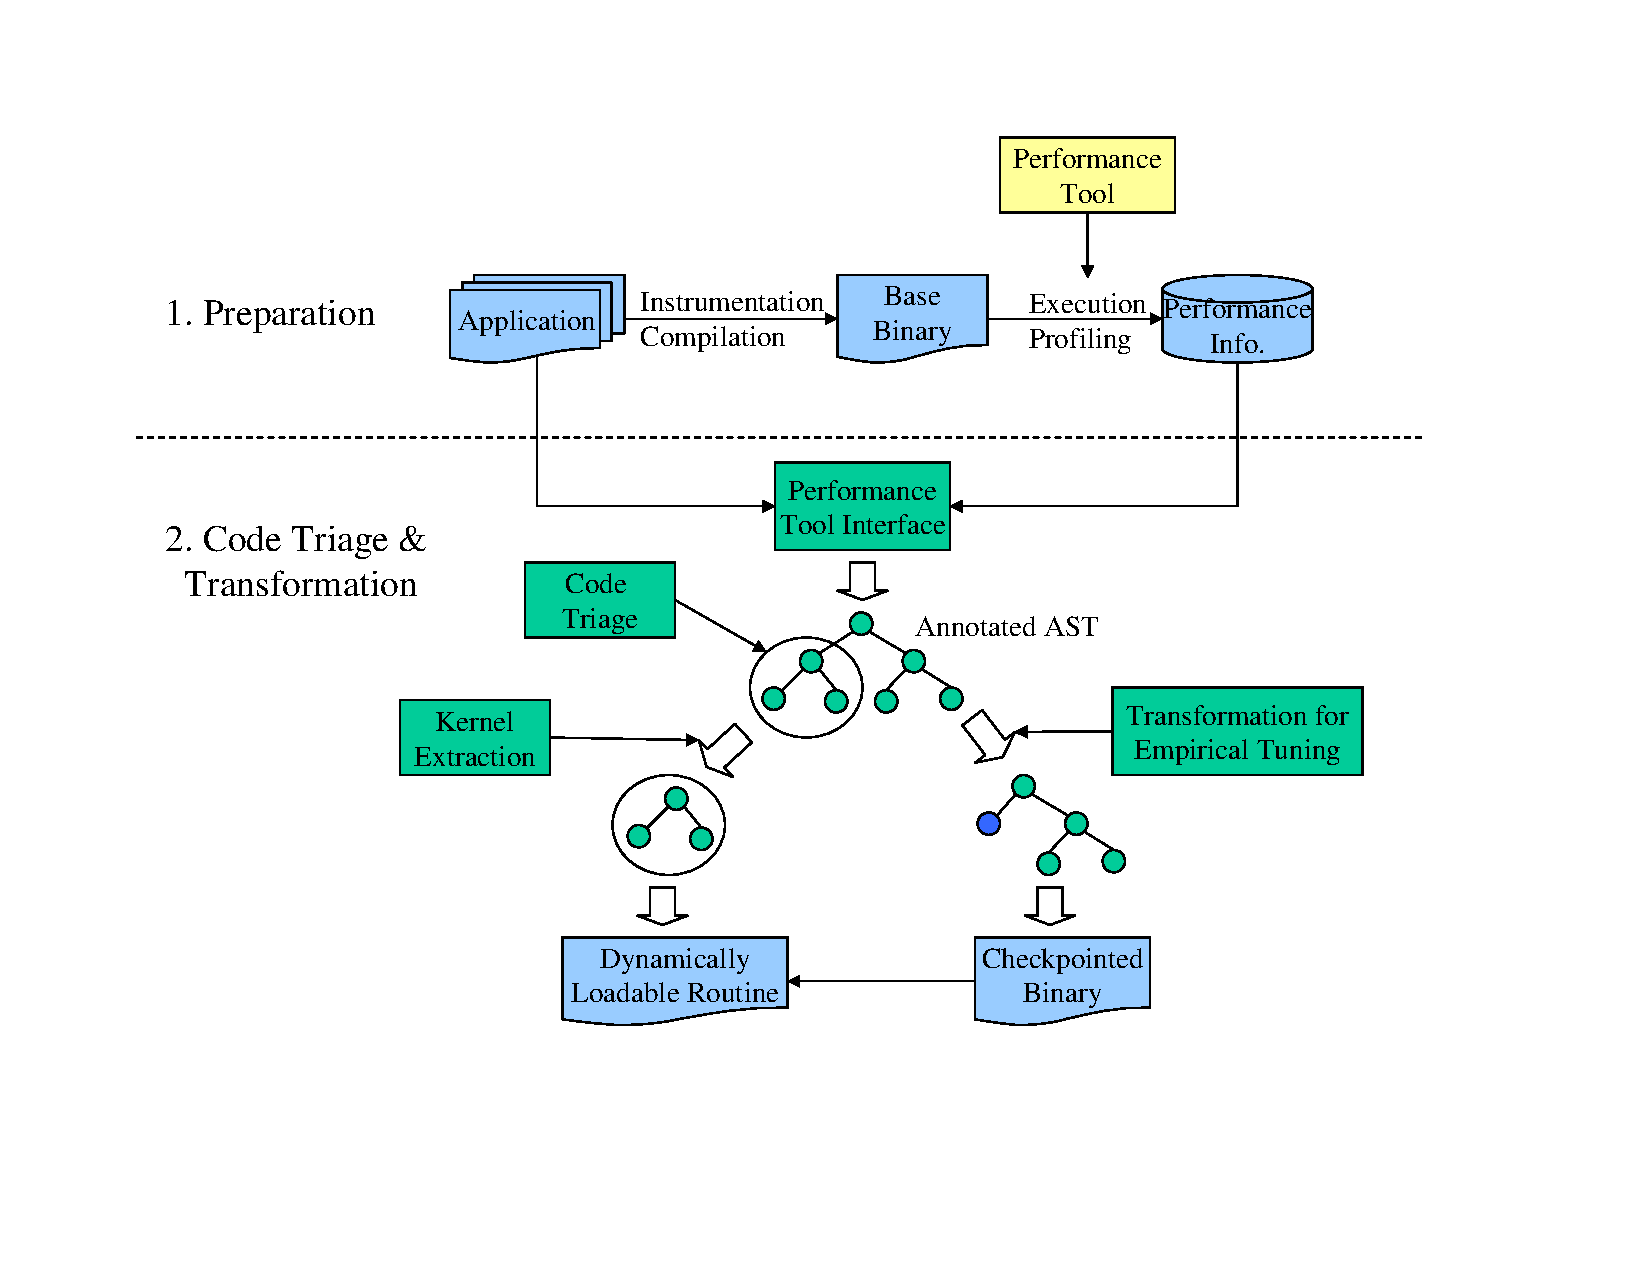
\includegraphics[width=1.2\textwidth]{phase12.pdf}
       \caption{Phase 1 and 2 of the autotuning system}
       \label{fig:phase12}
\end{figure}

%---------------------------------------------------
\subsection{Invoking Code Triage}
The source code for code triage is located in
\textit{rose/projects/autoTuning/autoTuning.C}. 
It already has initial implementation to call ROSE's tool interface,
conduct simple code triage, and finally extract kernels using ROSE's AST
outliner. 

With the input application and its performance result available, 
%a straightforward method is used to identify the most time-consuming
%statements in the code.  
%Loop nests containing those statements are reported as a
%tuning candidate, if the loop nests exist.
users can invoke the ROSE-based code triage by using the following command:

{\mySmallFontSize
\begin{verbatim}
autoTuning -c  jacobi.c -rose:hpct:prof jacobi-raw.xml \
-rose:autotuning:triage_threshold 0.8 -rose:outline:output_path "tests"
\end{verbatim}
}

The command above provides an input source file and its corresponding XML-format performance data generated by HPCToolkit.
It asks the code triage program to find the most time-consuming 
loops which account for just above 80\% of the total execution time. 
The identified loops will be automatically extracted to separated,
source files and saved into an output path named \textit{tests}.

Users can also enable code triage only without calling outlining. 
The performance data can come from GNU gprof. 
An example is given below:

%{\scriptsize
{\mySmallFontSize
\begin{verbatim}
# example command line to perform code triage only.
autoTuning  -c jacobi.c -rose:autotuning:triage_only -rose:gprof:linebyline jacobi.gprof.txt 

# the output is a list of abstract handles and 
# their corresponding execution time percentage
-----------------------------------------------------------------
The abstract handles for hot statements exceeding the threshold are:
Project<numbering,1>::SourceFile<name,/home/liao6/jacobi.c>::\
ExprStatement<position,193.9-194.76>
0.382
Project<numbering,1>::SourceFile<name,/home/liao6/jacobi.c>::\
ExprStatement<position,196.9-196.45>
0.3643
Project<numbering,1>::SourceFile<name,/home/liao6/jacobi.c>::\
ExprStatement<position,188.9-188.29>
0.11
-----------------------------------------------------------------
The abstract handles for enclosing loops for hot statements exceeding the
threshold are:
Project<numbering,1>::SourceFile<name,/home/liao6/jacobi.c>::\
ForStatement<position,190.5-198.7>
0.8189
\end{verbatim}
}

The above example command identifies a list of the most time-consuming statements and loops and reports them using abstract handles. 
The report will end once the sum of execution time of the statements or
loops reach or exceed a preset threshold (default is 75\% of the total execution time). 

We explain some details for the implementation of code triage and
autotuning-related transformations in the following subsections.
%----------------------------------------
\subsection{Tool Interface}
%A ROSE tool interface is required for understanding the performance results of each
%external performance tool. 
ROSE has a performance tool interface, called ROSE-HPCT,
in its distribution to accept performance results generated by external
performance tools .  
%Please follow the instructions from ROSE
%Tutorial's Chapter ROSE-HPCToolkit Interface to enable and use this module. 
Basically, it reads in the XML files generated from HPCToolkit and attaches performance metrics to
the ROSE AST representing the corresponding source code.
It can handle macro expansions during the metric match process.
When necessary, all performance metrics are also propagated from statement
levels to loop, function, and file levels. 
Similarly, it also accepts the line-by-line performance data generated by GNU
gprof.
%Currently, the ROSE-HPCToolKit interface is used to accept performance
%data generated by HPCToolkit and GNU gprof.
%The interface is used to annotate ROSE AST with performance metrics to
%facilitate building automated performance analysis tools. 
Detailed information about ROSE-HPCToolKit can be found in Chapter 44 of
the \htmladdnormallink{ROSE Tutorial}{http://www.rosecompiler.org/ROSE_Tutorial/ROSE-Tutorial.pdf}.
%We only give information relevant to autotuning below.

The code triage program uses the following code to invoke ROSE-HPCT.

{\mySmallFontSize
\begin{verbatim}
int main(int argc, char * argv[]) 
{
  vector<string> argvList (argv, argv+argc);
  // Read into the XML files
  RoseHPCT::ProgramTreeList_t profiles = RoseHPCT::loadHPCTProfiles (argvList);
  // Create the AST tree
  SgProject * project = frontend(argvList);
  //Attach metrics to AST , last parameter is for verbose
  RoseHPCT::attachMetrics(profiles, project,project->get_verbose()>0);
  //...
}
\end{verbatim}
}

%%----------------------------------------
%\subsection{Code Triage}
%A code triage module examines the AST annotated with
%performance metrics to locate problematic code portions (we call these code portions
%as autotuning targets).
%Currently, a straightforward top-down method is used to identify a hot spot
%in the code from the most time consuming file and then the loop nests containing such spot is reported as a
%tuning candidate, if the loop nests exist. The example code is shown below:
%\fixme{ROSE's AST merge could be used in the future to have a global view
%of AST merged from multiple source files.}
%
%{\mySmallFontSize
%\begin{verbatim}
% std::string hot_file = findHottestFile(fileMetrics);
% SgNode* hot_node=findHottestStatement(file, nodesWithMetrics);
% SgForStatement* target_loop= findTargetLoop(hot_node);
%
%\end{verbatim}
%}
%
%Code triage is also designed to suggest a set of potentially beneficial optimizations and
%their configuration ranges to improve the performance.
%\fixme{TODO need to implement this by compiler analysis. We manually 
% use the limited optimization choices, such as loop unrolling, by default for now.}
%
% DQ: Liao, what is the best entry point for me to write such a module/traversal.
% I think it would be good to have this in place before we release this document.
% I will be happy to write this part.

%----------------------------------------
\subsection{Kernel Extraction: Outlining}
Each of the identified tuning targets, often loops, will be extracted from the original code to
form separated functions (or routines). 
The ROSE AST outliner is invoked to generate such functions. 
%It replaces a block of consecutive statements with a function call to a newly generated
%function containing those statements. 
This kernel extraction step can be automatically invoked by the code triage
program or manually initiated by users via the outliner's command line
interface. 

The ROSE AST outliner handles multiple input languages, including C, C++ and
recently Fortran.  It also provides both command line and programming interfaces for users
to specify the targets to be outlined.  
Detailed information of using the ROSE outliner can be found in
Chapter 27 of the \htmladdnormallink{ROSE
Tutorial}{http://www.rosecompiler.org/ROSE_Tutorial/ROSE-Tutorial.pdf}.
You can also refer to a paper~\cite{LiaoEffective2009} for the algorithm we use to outline kernels. 
%More details of the ROSE AST outliner are
%available in the ROSE Tutorial's Chapter, Function Outlining using the AST Outliner.
For the code triage program, the programming interface of the Outliner is
used as below:

{\mySmallFontSize
\begin{verbatim}
  // recognize options for outliner
  Outliner::commandLineProcessing(argvList);
  ...
 SgForStatement* target_loop= findTargetLoop(hot_node);
 if (isOutlineable (target_loop))  
   outline(target_loop);
\end{verbatim}
}

The ROSE AST outliner accepts user options to further guide its internal
behavior. \lstinline{-rose:outline:parameter_wrapper } will wrap all
parameters of the outlined function into an array of pointers. 
\lstinline{-rose:outline:new_file} will separate the outlined function into
a new source file to facilitate external tools for further handling.
\lstinline{-rose:outline:use_dlopen} will transform the code to use
\lstinline{dlopen()} and \lstinline{dlsym()} to dynamically load the
outlined function from a library.

For the SMG2000 example, the most time-consuming loop is outlined and a call to it is used
to replace the loop in the original code. 
The loop is actually expanded from a macro
\lstinline{hypre_BoxLoop3For()}. 
ROSE is able to identify it after a bottom
up metrics propagation phase in ROSE-HPCT. 
%\fixme{Need to come up a way to automatically handle this, Should we
%do it within the outliner itself or before calling the outliner?})
The kernel extraction's result is shown in the following code listing:
\lstset{language={C},basicstyle=\scriptsize} 
\lstinputlisting{smg2000_outlined.fold.c}
\lstset{language={C},basicstyle=\small} 

%\fixme{TODO 
%   Also we should evaluate the overhead of this
%   step if the final result is an optimized function represented as a separate 
%   file (potentially disables some optimizations).  In the final assembly 
%   we could remove the dynamic linking, but the Makefile would have to be modified which
%   gets messy for an automated system.}

The ROSE outliner uses a variable cloning method to
avoid using pointer dereferencing within the outlined computation kernels. 
The method is based on usage of a variable that is passed by reference and
accessed
via pointer-dereferencing by classic outlining algorithms.
Such a variable is used either by value or by address within an outlining
target.
For the C language, using the variable by address occurs when the
address operator
is used with the variable (e.g. \lstinline{&X}).
C++ introduces one more way of using the variable by address:
associating the variable with a reference type
(\lstinline{TYPE & Y = X;} or using the variable as an argument for a
 function's parameter of a reference type).
If the variable is not used by its address,
a temporary clone variable of the same type (using \lstinline{TYPE clone;})
can be introduced to substitute its uses within the outlined function.
The value of a clone has to be
initialized properly (using \lstinline{clone = * parameter;})
before the clone participates in computation.
After the computation, the original variable must be set to the clone's
final value
(using \lstinline{*parameter = clone}).
By doing this, many pointer dereferences introduced by the classic
algorithm can be avoided.
\fixme{We are working on using liveness analysis to further eliminate unnecessary
value assignments.}

For easier interaction with other tools, the outlined function is separated
into a new source file, usually named after 
the function name.  
The ROSE outliner will recursively find and copy all dependent type declarations
into the new file to make it compilable.
For the SMG2000 example, a file named out\_1\_6755\_\_.orig.c 
is generated and it only contains the function body of \lstinline{OUT_1_6755__()}. 
This file will be transformed by a parameterized optimizer to a kernel
variant named OUT\_\_1\_\_6755\_\_.c and further compiled into a dynamically
loadable routine.

A sample makefile to generate the .so file is given below: 

{\mySmallFontSize
\begin{verbatim}
[liao@localhost smg2000] cat makefile-lib
lib:OUT__1__6755__.so
OUT__1__6755__.o:OUT__1__6755__.c
        gcc -c -fpic OUT__1__6755__.c
OUT__1__6755__.so:OUT__1__6755__.o
        gcc -shared -lc -o OUT__1__6755__.so OUT__1__6755__.o
clean:
        rm -rf OUT__1__6755__.so OUT__1__6755__.o
\end{verbatim}
}

%----------------------------------------
\subsection{Transformations for Autotuning}
The call site of the outlined function in the source code has to be further transformed to support empirical optimization. 
These transformations include:
\begin{itemize}
\item using \lstinline{dlopen()} to open a specified .so file containing
the outlined target and calling the function found in the file,
\item adding performance measuring code to time the call of the outlined target function.
\item transforming code to support checkpointing the execution right before
\lstinline{dlopen()} opening the library source file so multiple variants of the file can be used to test optimization choices empirically when the program is restarted multiple times.
\end{itemize}
%\fixme{TODO the code translations in this sub section are manually done
%now. We will start to
%implement them once the translation methods are agreed on by partners.}
%----------------------------------------
\subsubsection{Calling a Function Found in a .so File}
As mentioned earlier, the outlined function containing the target kernel is
stored in a separated source file, which will be transformed into a kernel variant
and then compiled to a dynamically loadable library. 
The original source code has to be transformed to open the library file,
find the outlined function, and finally call it using the right
parameters. An example of the resulting transformation on the function containing the
outlined loop is given below:
\lstset{language={C}, basicstyle=\scriptsize}
\lstinputlisting{smg2000_dlopen.c}

\subsubsection{Timing the Call}
The call to the outlining target kernel should be timed to get the
evaluation results during the empirical optimization. 
We instrument the call as follows to get the performance evaluation of a
kernel variant. 
More accurate and less intrusive methods based on hardware
counters can also be used in the future. 

{\mySmallFontSize
\begin{verbatim}
//save timing information into a temporary file

remove("/tmp/peri.result");
time1=time_stamp();
// parameter wrapping statements are omitted here
(*OUT__1__6755__)(__out_argv1__1527__);

time2=time_stamp();
FILE* pfile;
pfile=fopen("/tmp/peri.result","a+");
if (pfile != NULL)
{
  fprintf(pfile,"%f\n",time2-time1);
  fclose(pfile);
}
else
  printf("Fatal error: Cannot open /tmp/peri.result!\n");

\end{verbatim}
}

%----------------------------------------
\subsubsection{Checkpointing and Restarting}
In order to efficiently evaluate hundreds or even thousands of kernel
variants, we use a checkpointing and restarting method to measure the time
spent on calling the kernel without unnecessarily repeating the execution
before and after calling the kernel.  This allows the full context (state) 
of the application to be used in the evaluation of the kernel performance.
\fixme{need to discuss the drawbacks, e.g. missing cache warmup; and how that
might be addressed in the future by pushing back the checkpoint start and 
transformations to the checkpointed program (later).}

The Berkeley Lab Checkpoint/Restart (BLCR) library~\cite{blcrWeb} was selected for its
programmability, portability and robustness. 
BLCR is designed to support asynchronous checkpointing, which means a running process
is notified by another process to be checkpointed first, but the exact checkpointing
action happens on an indeterministic point later on. 
This default behavior is not desired for our purpose since we want an
accurate source position to do the checkpointing. 
Fortunately, BLCR's library does provide some internal functions to help
us initiate synchronous (immediate) checkpointing, though not well documented. 
After some trial and error rounds, we use the following code transformation
to have a synchronous checkpointing using the blcr-0.8.2 release.
The idea is to have a running program to notify itself to initiate a checkpointing. 
The program is then blocked until the request is served. 

To support BLCR, we have transformed the original source code in two locations.
% Two places in the source files have to be changed. 
The first location is the file where the main() function exists. We add the necessary
header files and initialization codes for using BLCR.  For example:
\lstset{language={C}, basicstyle=\scriptsize}
\lstinputlisting{smg2000_checkpoint.c}
% \lstset{language={C}, basicstyle=\small}

The second place is the actual source line to initiate the checkpointing. 
A checkpoint argument structure is filled out first to customize the
behavior we want, including the scope, target, memory dump file,
consequence, and so on. A blocking phase is put right after
\lstinline{cr_request_checkpoint()} to have an immediate checkpointing.
Our goal is to stop the executable right before opening the .so file so
a different kernel variant can be compiled into the .so file each time. 
The execution will be restarted multiple times so multiple variants can 
be evaluated this way. 

\lstset{language={C}, basicstyle=\scriptsize}
\lstinputlisting{smg2000_checkpoint2.c}
% \lstset{language={C}, basicstyle=\small}

Only these minimum transformations are needed to build the target application to support
BLCR. We choose the static linking method to support BLCR as follows.
The BLCR library is linked with the final executable. 

{\mySmallFontSize
\begin{verbatim}
smg2000: smg2000.o
        @echo  "Linking" \$@ "... "
        \${CC} -o smg2000 smg2000.o \${LFLAGS} -lcr
\end{verbatim}
}

The checkpointed binary has to be executed once to generate a memory dump
file (process image), which can then be reused multiple times to restart the execution 
immediately before the line where \lstinline{dlopen()} is invoked to evaluate multiple
variants of the optimization target kernel.

{\mySmallFontSize
\begin{verbatim}
[liao@localhost test] ./smg2000 -n 120 120 120 -d 3
current process ID is 6028
Running with these driver parameters:
  (nx, ny, nz)    = (120, 120, 120)
  (Px, Py, Pz)    = (1, 1, 1)
  (bx, by, bz)    = (1, 1, 1)
  (cx, cy, cz)    = (1.000000, 1.000000, 1.000000)
  (n_pre, n_post) = (1, 1)
  dim             = 3
  solver ID       = 0
=============================================
Struct Interface:
=============================================
Struct Interface:
  wall clock time = 0.550000 seconds
  cpu clock time  = 0.540000 seconds
Checkpoiting: stopping here ..
Killed
\end{verbatim}
}

A context dump file named dump.yy will be generated by BLCR as the
checkpointing result. This dump file will be used to restart the execution using
the command: \lstinline{cr_restart dump.yy}.

\section{Empirical Tuning}
The actual empirical tuning (shown in Fig.~\ref{fig:phase3}) is conducted via the cooperation of several
components: a search engine, a parameterized transformation tool, and 
the previously introduced checkpointing/restarting library.
The basic idea is that:
1) a set of pre-selected transformations and their corresponding configuration
   ranges are given (by the code triage module) and converted into an integral
   search space; 
2) the search engine evaluates points from the search space by driving the parameterized
   transformation tool to generate kernel variants and restarting the checkpointed binary
   to run the variants one by one.
\begin{figure}[htbp]
       \centering
               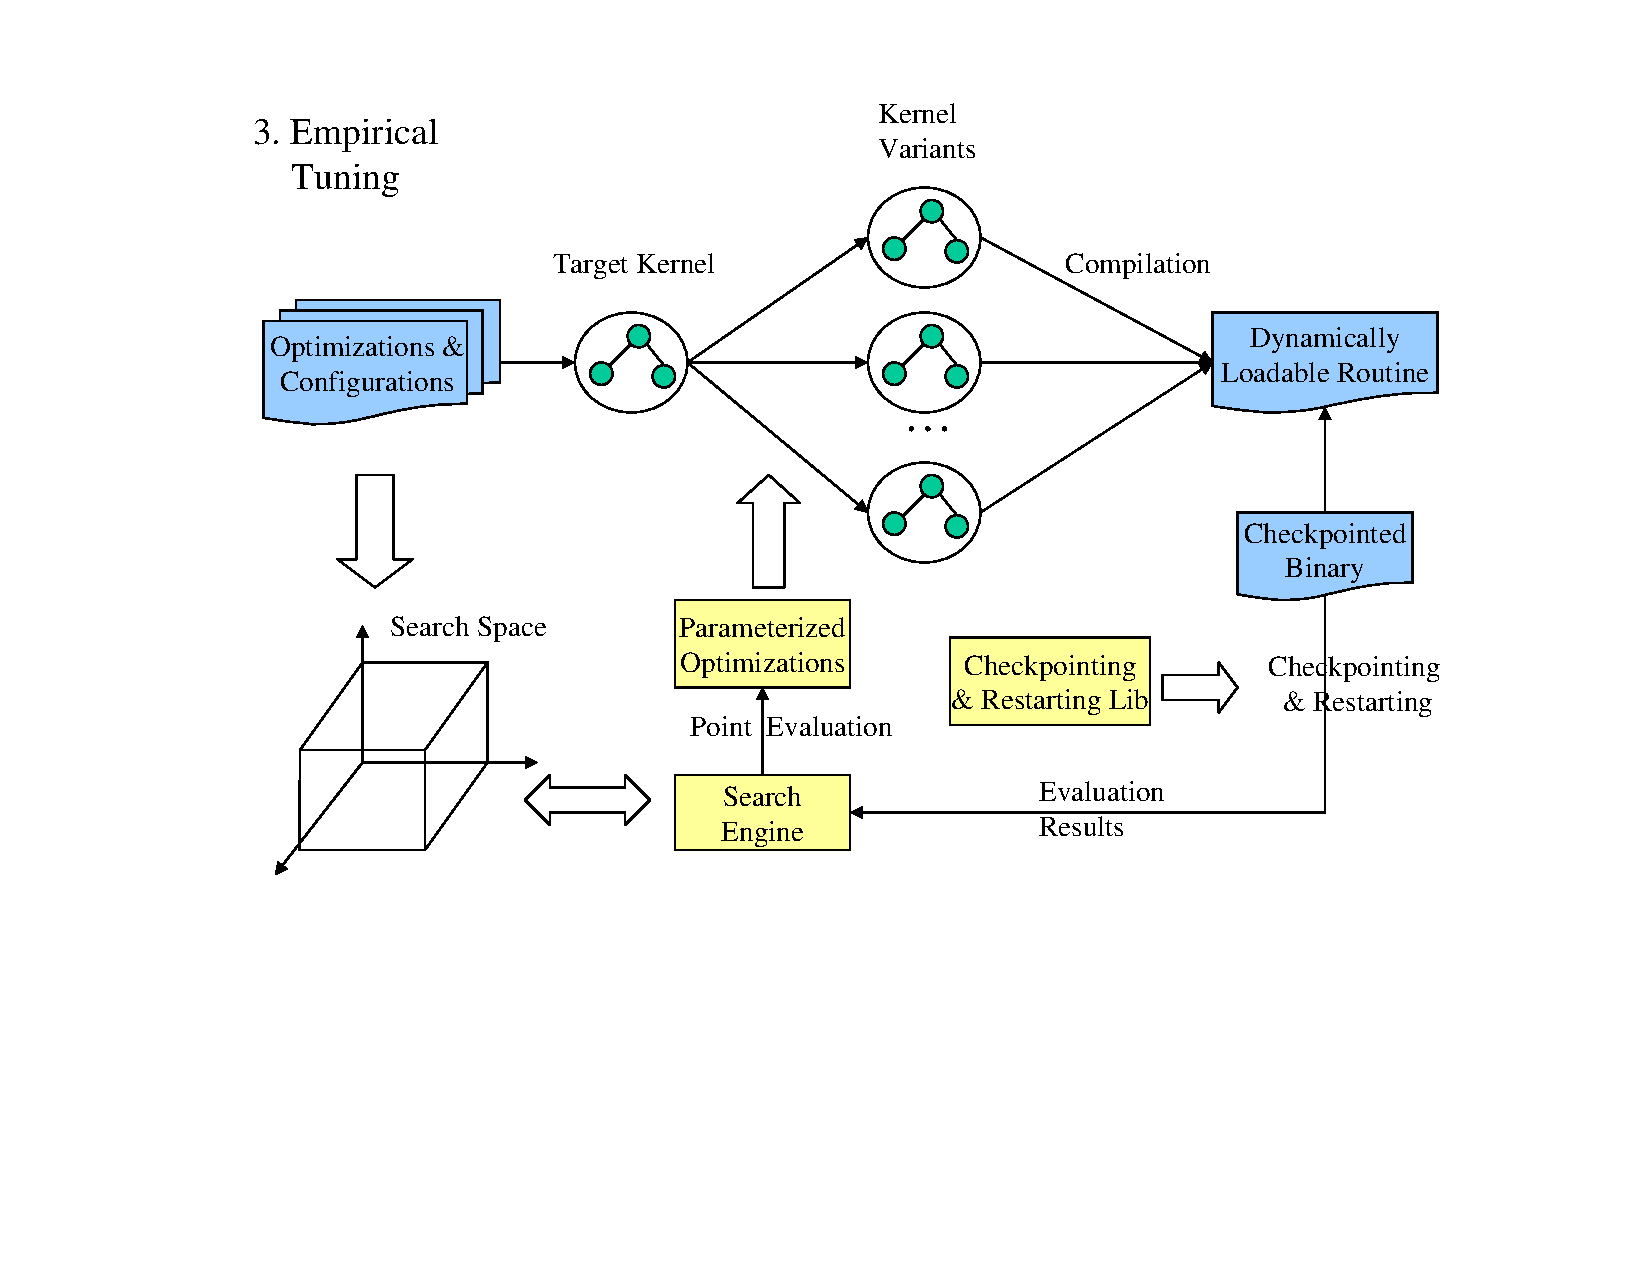
\includegraphics[width=1.2\textwidth]{phase3.pdf}
       \caption{Phase 3 of the autotuning system}
       \label{fig:phase3}
\end{figure}

%--------------------------------------------------
\subsection{Parameterized Transformation Tools}
Several choices exist to generate kernel variants, they include
POET~\cite{YiPOET2007},
CHiLL~\cite{ChenCHiLL2008}, and the ROSE loop translators. We take POET as an example here. 

POET (Parameterized Optimizations for Empirical
Tuning) developed by Dr.~Qing~Yi under contract with University of
Texas at San Antonio (UTSA), is an efficient language and tool to express hundreds or
thousands of complex code transformations and their configurations using a small set
of parameters.  It is especially relevant to the evaluation of large-scale search spaces
as part of empirical tuning and is orthogonal to any specific search strategy.

Using command line options and a configuration file, users can direct POET to apply a set
of specified transformations with desired configurations on selected code portions. 
Also, the target kernel has to be instrumented to aid POET in the process. 
Detailed POET user instructions can be found at its official website~\cite{poetWeb}.
For example, the SMG2000 kernel has the following format to support
POET:
\begin{figure}[!ht]
\centering
\lstset{language=C, basicstyle=\scriptsize}
\begin{lstlisting}
void
OUT__1__6755__ (void **__out_argv)
{
  int Ai =  *((int *)(__out_argv[20]));
  int xi =  *((int *)(__out_argv[19]));
  int ri =  *((int *)(__out_argv[18]));
  double *Ap =  *((double **)(__out_argv[17]));
  double *xp =  *((double **)(__out_argv[16]));
  double *rp =  *((double **)(__out_argv[15]));
  int loopi =  *((int *)(__out_argv[14]));
  int loopj =  *((int *)(__out_argv[13]));
  int loopk =  *((int *)(__out_argv[12]));
  int hypre__sx1 =  *((int *)(__out_argv[11]));
  int hypre__sy1 =  *((int *)(__out_argv[10]));
  int hypre__sz1 =  *((int *)(__out_argv[9]));
  int hypre__sx2 =  *((int *)(__out_argv[8]));
  int hypre__sy2 =  *((int *)(__out_argv[7]));
  int hypre__sz2 =  *((int *)(__out_argv[6]));
  int hypre__sx3 =  *((int *)(__out_argv[5]));
  int hypre__sy3 =  *((int *)(__out_argv[4]));
  int hypre__sz3 =  *((int *)(__out_argv[3]));
  int hypre__nx =  *((int *)(__out_argv[2]));
  int hypre__ny =  *((int *)(__out_argv[1]));
  int hypre__nz =  *((int *)(__out_argv[0]));
  for (loopk = 0; loopk < hypre__nz; loopk+=1) 
  {
    for (loopj = 0; loopj < hypre__ny; loopj+=1) 
    {
      for (loopi = 0; loopi < hypre__nx; loopi+=1)  //@BEGIN(nestI)
      {
        {
          rp[ri] -= ((Ap[Ai]) * (xp[xi]));
        }
        Ai += hypre__sx1;
        xi += hypre__sx2;
        ri += hypre__sx3;
      }
      Ai += (hypre__sy1 - (hypre__nx * hypre__sx1));
      xi += (hypre__sy2 - (hypre__nx * hypre__sx2));
      ri += (hypre__sy3 - (hypre__nx * hypre__sx3));
    }                                             //@END(nestI:Nest)
    Ai += (hypre__sz1 - (hypre__ny * hypre__sy1));
    xi += (hypre__sz2 - (hypre__ny * hypre__sy2));
    ri += (hypre__sz3 - (hypre__ny * hypre__sy3));
  }
 // some code omitted here...
}
\end{lstlisting}
  \caption{the SMG 2000 kernel}
    \label{Fig:smg2000kernel}
\end{figure}
%  for (loopk = 0; loopk < *hypre__nz; loopk+=1)
%    {
%      for (loopj = 0; loopj < *hypre__ny; loopj+=1)
%        {
%          for (loopi = 0; loopi < *hypre__nx; loopi+=1) //@BEGIN(nestI)
%            {
%              {
%                (*rp)[*ri] -= (((*Ap)[*Ai]) * ((*xp)[*xi]));
%              }
%              *Ai += *hypre__sx1;
%              *xi += *hypre__sx2;
%              *ri += *hypre__sx3;
%            }                                               //@END(nestI:Nest)
%          *Ai += (*hypre__sy1 - (*hypre__nx * *hypre__sx1));
%          *xi += (*hypre__sy2 - (*hypre__nx * *hypre__sx2));
%          *ri += (*hypre__sy3 - (*hypre__nx * *hypre__sx3));
%        }
%      *Ai += (*hypre__sz1 - (*hypre__ny * *hypre__sy1));
%      *xi += (*hypre__sz2 - (*hypre__ny * *hypre__sy2));
%      *ri += (*hypre__sz3 - (*hypre__ny * *hypre__sy3));
%    }
 
\fixme{TODO:the input is manually changed from the kernel generated by
the autoTuning translator. POET expects normalized loops
with special tags, integer loop control variables and $++$ operator is not allowed. 
We will discuss with Qing to either drop these restrictions or use ROSE to normalize
the loops automatically.}

The POET configuration file (my.pt) we use to optimize SMG2000's kernel is shown
below. In this file, loop unrolling is specified to be performed on the target
within a source file named out\_1\_6755\_\_.org.c. 
The result will be saved inside a file named out\_1\_6755\_\_c.
\lstset{basicstyle=\scriptsize}
\lstinputlisting{my.pt.fold}

A default transformation parameter, unrolling factor, is also given in the
file. But this parameter is usually superseded by a command line
parameter, the following command line specifies unrolling 5 times.
%The extracted kernel will be compiled as a dynamically loadable routine to
%be used by the target application. 
{\mySmallFontSize
\begin{verbatim}
/home/liao/download/qing/POET/src/pcg -punrollI=5 \
-L/home/liao/download/qing/POET/lib my.pt 
\end{verbatim}
}

\fixme{TODO The generation of .pt files it not yet automated currently.}

%--------------------------------------------------
\subsection{Search Engines}
Currently, we adopt the GCO (Generic Code Optimization) search engine~\cite{Youeffective2005} from University of Tennessee
at Knoxville as the external search engine used in our system.  
It has been connected with
a specific version of POET (not yet fully updated to the latest POET release
unfortunately) to explore code transformations using several popular search policies,
such as random search, exhaustive search, simulated anneal search, genetic algorithm,
and so on.

The search engine interacts with the parameterized optimization tool (POET)
via a bash script, usually named as eval\_xxx where xxx indicates the
target application.
This script is manually generated currently and does the following tasks:
\begin{enumerate}
   \item specifies the search space's dimension number and lower, upper bound
         for each dimension,
   \item specifies the number of executions for each evaluation. This will
         help exclude some executions disturbed by system noises, 
   \item validation of the number of command line options for this script, the
         number should match the number of dimensions of the search space so each
         value corresponding one dimension. All the options together mean a valid
         search point within the search space.
   \item converts the search point into transformation parameters
         understandable by POET. Some transformation choices are obtained by
         interpreting integer values in a custom way, such as the order of loop interchanging. 
   \item generates a kernel variant by invoking POET with right parameters to conduct the
         corresponding transformations on the target kernel,
   \item compiles the generated kernel variant into a dynamically loadable
         shared library file (a .so file),
   \item restarts the checkpointed binary to evaluate the kernel variant. This step is
         repeated multiple times as configured and the shortest execution time is reported as
         the evaluation result for this particular transformation setting (a point).
\end{enumerate}

A full example script for SMG2000 is given below.
\lstset{basicstyle=\scriptsize}
\lstinputlisting{eval_smg.fold}
\lstset{basicstyle=\small}

As we can see, the evaluation of a kernel variant needs the cooperation of
three parties.
\begin{enumerate}
   \item the transformed target application providing a performance
         measurement (timing) for the call to the variant, 
   \item the \lstinline{eval_smg} script choosing the best execution after
         several times of execution using the same kernel variant,
   \item the search engine retrieving the information returned from
         \lstinline{eval_smg} as the evaluation result of a variant and proceeding
         the search accordingly.
\end{enumerate}

%---------------------------------------------------------------
\subsection{An Example Search}
   We use the random search policy of the UTK search engine to demonstrate a
sample search process. The search engine chooses the maximum evaluation value as the best
result by default. So a reciprocal of a timing result is indicated by an environment
variable \lstinline{GCO_SEARCH_MODE} to be the evaluation result.  The UTK search engine
also accepts a upper time limit for a search session.  We use 1 minute in this example by
adding 1 as the last parameter. 
%following \lstinline{eval_smg}.

{\mySmallFontSize
\begin{verbatim}
[liao@localhost smg2000]$ export GCO_SEARCH_MODE=reciprocal
[liao@localhost smg2000]$ ../search/random_search ./eval_smg 1
Checkpointing: restarting here ..
Case: ./eval_smg 12  --
Got the evaluation result: 50.7846
Checkpointing: restarting here ..
Case: ./eval_smg 13  --
Got the evaluation result: 49.65
Checkpointing: restarting here ..
Case: ./eval_smg 11  --
Got the evaluation result: 50.9502
Checkpointing: restarting here ..
Case: ./eval_smg 31  --
Got the evaluation result: 49.8107
Checkpointing: restarting here ..
Case: ./eval_smg 15  --
Got the evaluation result: 49.8703
Checkpointing: restarting here ..
Case: ./eval_smg 14  --
Got the evaluation result: 49.645
Checkpointing: restarting here ..
Case: ./eval_smg 25  --
Got the evaluation result: 50.0551
Checkpointing: restarting here ..
Case: ./eval_smg 18  --
Got the evaluation result: 49.7018
skipping already visited point 31 , value = 49.810719
Checkpointing: restarting here ..
Case: ./eval_smg 32  --
Got the evaluation result: 49.5221
Checkpointing: restarting here ..
Case: ./eval_smg 22  --
Got the evaluation result: 49.6475
Checkpointing: restarting here ..
Case: ./eval_smg 6  --
Got the evaluation result: 51.261
Checkpointing: restarting here ..
Case: ./eval_smg 30  --
Got the evaluation result: 50.0475
skipping already visited point 18 , value = 49.701789
skipping already visited point 14 , value = 49.645038
Checkpointing: restarting here ..
Case: ./eval_smg 4  --
Got the evaluation result: 51.435
Time limit reached...
---------------------------------------------------
Random Search Best Result:  Value=49.522112, Point=32
Total Number of evaluations: 13

\end{verbatim}
}

In the sample search above, a one-dimension search space (loop unrolling
factor) was examined.  
Within the one-minute time limit, points were randomly chosen by the
search engine and three of them were redundant. 
Apparently, the UTK search engine was able to skip redundant evaluations.
In the end, a point (32) had the best value (reciprocal of timing) which
means for the target smg2000 kernel, unrolling 32 times generated the best
performance.

Similarly, other search policies can be used by replacing
\lstinline{random_search} with
\lstinline{exhaustive_search}, \lstinline{anneal_search},
\lstinline{ga_search}, \lstinline{simplex_search}, etc. 

\section{Working with Active Harmony}
We describe how our end-to-end empirical tuning framework can be adapted to work with another search engine, namely the Active Harmony system~\cite{TapusActive2002,ChungCase2006}. 
The work is done with generous help from Ananta Tiwari at University of
Maryland.

Active Harmony allows online, runtime tuning of application parameters which are critical to the application performance. 
Domain-specific knowledge is usually needed to identify those application parameters.
An active harmony server will be running to manage the values of different application parameters and to conduct the search.
Applications have to be modified to communicate with the server in order to send performance feedback for one specific set of parameter values (current point) and get the next set of parameter values (next point).
Currently, it supports a search strategy based on the Nelder-Mead simplex method~\cite{NelderSimplex1965}.

For SMG2000, we generate a set of unrolled versions (OUT\_\_1\_\_6755\_\_X()) for the target kernel and treat the function suffix X as the tunable parameter. 
As a result, the .so file contains all unrolled versions.
\fixme{This is not an ideal way to tune the application, we will explore better alternatives.}

%TODO add the tcl configuration file here
A configuration file is needed for Active Harmony to know the parameters to
be tuned and their corresponding ranges. 
The following file is used to specify a tunable parameter named unroll with a range from 1 to 32.
obsGoodness (observed Goodness - or performance) and predGoodness (predicted goodness) are related to a GUI window showing during the execution. 
They do not impact the performance tuning and the workings of the search algorithm. 
{\mySmallFontSize
\begin{verbatim}
harmonyApp smg2000Unroll {
   { harmonyBundle unroll {
       int {1 32 1}
   }
   }
    { obsGoodness 1 5000}
    { predGoodness 1 5000}
}
\end{verbatim}
}

We don't use BLCR since an online tuning method is used for Active Harmony. 
The code transformation to work with Active Harmony is shown below.
The basic idea is to call a set of Harmony interface functions to startup communication with the server (\lstinline{harmony_startup()}),
send a configuration file (\lstinline{harmony_application_setup_file()}), define a parameter to be tuned (\lstinline{harmony_add_variable(})),  report performance feedback (\lstinline{harmony_peformance_update()}), 
and finally request the next set of values of the tunable parameters (\lstinline{harmony_request_all()}).
\lstset{language={C},basicstyle=\scriptsize}
\lstinputlisting{smg2000_harmony.c}
\lstset{language={C},basicstyle=\small}

Figure~\ref{fig:activeHarmony2} shows a screen shot of using Active Harmony to tuning the SMG2000 benchmark. 
The top panel gives a graphical representation of the search space (one dimension named unroll) and the tuning timeline with evaluation values (x-axis is time, y-axis is evaluation values). 
The left-bottom shell window is the client application being tuned. 
The right-bottom shell windows shows the activities of the server.
\begin{figure}[tbp]
        \centering
                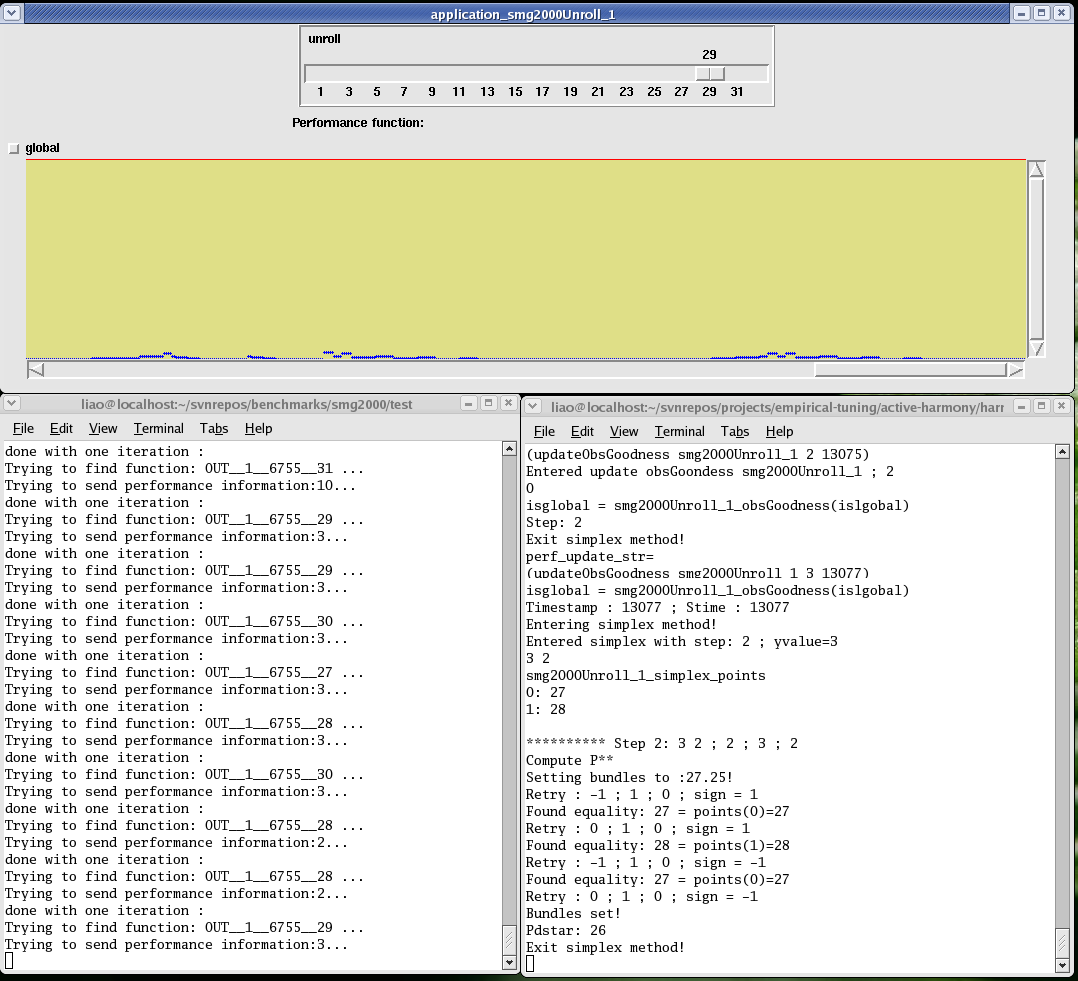
\includegraphics[width=0.8\textwidth]{activeHarmony2.png}
        \caption{Searching using Active Harmony}
        \label{fig:activeHarmony2}
\end{figure}

We have found that online/runtime search engines like the Active Harmony can be extremely expensive if the tuned kernel are invoked thousands of times. 
For SMG2000, it took hours to finish the tuning using a 120x120x120 input data set.
The major reason is that for each call of the kernel, a bidirectional communication between the client application and the server has to be finished. 
Another reason is that the current tuning process is embedded into the thousands of calls of the kernel so that points are always evaluated even when some of them have already been evaluated before. 



\section{Summary}

   The work presented is ongoing work, and focused on the whole program empirical tuning
and the automation of all the required steps to make that work for realistic HPC applications
in C, C++, and Fortran.  
The work to has a few steps that are likely not so easy to fully
automate, namely the manipulation of the Makefiles and bash scripts that are required to support the empirical
tuning, but it is likely this can be simplified in the future.

The work presented is also immediately focused on providing an infrastructure for 
the empirical tuning and less on the empirical tuning of any specific applications.
SMG2000 was selected somewhat at random, since it is moderately large and 
we have demonstrated for many years that we can compile it easily with ROSE.


% just put it here temporarily

\chapter{ Appendix }

%  Purpose:
% \begin{itemize}
%    \item A. Error messages
%    \item B. How to add new IR nodes (prep for F90 work with Rice)
% \end{itemize}
% \begin{center}
% *********************  \newline
% \end{center}
% \vspace{0.25in}
% 
%     Put text here!

   This appendix covers a number of relavant topics to the use of ROSE
which have not been worked into the main body of text in the ROSE User Manual.

\fixme{ The sections within this Appendix are staged here while we figure out where they
        belong in the ROSE User Manual (or elsewhere).}

% DQ: Until we have error message we can ignore this section (suggested by Rich)
\section {Error Messages}

   The user will mostly only see error messages from EDG, these will
appear like normal C++ compiler error messages.

   These can be turned off using the edg option: \\
   --edg:no\_warnings \\
or \\
   -edg:w \\
on the command-line of any translator built using ROSE.

\section {Specifying EDG options}

   The EDG options are specified using --edg:$<$edg option$>$ for edg options starting 
with "--" or -edg:$<$edg option$>$ for edg options starting with "-".

The details of the EDG specific options are available at: \\
    http://www.edg.com/docs/edg\_cpp.pdf
available from the EDG web page at:\\
    http://www.edg.com/cpp.html

\section{Easy Mistakes to Make: How to Ruin Your Day as a ROSE Developer}

   There are a few ways in which you can make mistakes within the development of
the ROSE project:

\begin{enumerate}
     \item Never run {\tt configure} in your source tree.  If you do, then never run 
     {\tt make distclean}, since this will remove many things required to develop 
     ROSE. Things removed by {\tt make distclean} are:
     \begin{enumerate}
          \item documentation (including several of the directories in {\tt ROSE/docs/Rose})
     \end{enumerate}
\end{enumerate}

\section{Handling of source-filename extensions in ROSE}
    On case-sensitive systems, ROSE handles .c as the (only) valid filename extension
for c-language and .cc, .cp, .c++, .cpp, .cxx, as the valid filename extensions for
C++ language. On case-insensitive systems, ROSE handles .c and .C as valid filename
extensions for c-language, and .cc, .cp, .c++, .cpp, .cxx, .CC,
.CP, .C++, .CPP, .CXX as valid filename extensions for C++.

There are some inconsistencies in the filename handler such as: (1) not recognizing
.CC, .CP, .C++, .CPP, .CXX as valid filename extensions for C++ language on case-sensitive
systems and  (2) not recognizing .CxX, .cPp, etc. as valid filename extensions for
C++ language on case-sensitive systems. The sole reason for the inconsistency is that
of compatibility with GNU (as well as EDG).


\section{IR Memory Consumption}
    The Internal Representation is used to build the AST and, for large programs,
it can translate into a large number of IR nodes.  Typically the total number of 
IR nodes is about seven times the number of lines of codes (seems to be a general 
rule, perhaps a bit more when templates are used more dominantly).  The memory
consumption of any one file is not very significant, but within support for whole
program analysis, the size of the AST can be expected to be quite large.  Significant
sharing of declarations is made possible via the AST merge mechanisms.  C and C++
have a One-time Definition Rule (ODR) that requires definitions be the same
across separate compilations of files intended to be linked into a single application.
ODR is significantly leveraged within the AST merge mechanism to share all declarations
that appear across multiple merged files.  Still, a one-million line C++ application 
making significant use of templates can be expected to translate into 10-20 million 
IR nodes in the AST, so memory space is worth considering.

   The following is a snapshot of current IR node frequency and memory consumption for
a moderate 40,000 line source code file (one file calling a number of header files).
% The AST contains a total of 
Note that the Sg\_File\_Info IR nodes are most frequent and consume the greatest amount 
of memory. This reflects our bias toward preserving significant information about the
mapping of language constructs back to the positions in the source file to support
a rich set of source-to-source functionality.

{\mySmallestFontSize
\begin{verbatim}
AST Memory Pool Statistics: numberOfNodes = 114081 memory consumption = 5019564 node = Sg_File_Info
AST Memory Pool Statistics: numberOfNodes =  31403 memory consumption =  628060 node = SgTypedefSeq
AST Memory Pool Statistics: numberOfNodes =  14254 memory consumption =  285080 node = SgStorageModifier
AST Memory Pool Statistics: numberOfNodes =  14254 memory consumption = 1140320 node = SgInitializedName
AST Memory Pool Statistics: numberOfNodes =   8458 memory consumption =  169160 node = SgFunctionParameterTypeList
AST Memory Pool Statistics: numberOfNodes =   7868 memory consumption = 1101520 node = SgModifierType
AST Memory Pool Statistics: numberOfNodes =   7657 memory consumption =  398164 node = SgClassType
AST Memory Pool Statistics: numberOfNodes =   7507 memory consumption = 2071932 node = SgClassDeclaration
AST Memory Pool Statistics: numberOfNodes =   7060 memory consumption =  282400 node = SgTemplateArgument
AST Memory Pool Statistics: numberOfNodes =   6024 memory consumption =  385536 node = SgPartialFunctionType
AST Memory Pool Statistics: numberOfNodes =   5985 memory consumption = 1388520 node = SgFunctionParameterList
AST Memory Pool Statistics: numberOfNodes =   4505 memory consumption = 1477640 node = SgTemplateInstantiationDecl
AST Memory Pool Statistics: numberOfNodes =   3697 memory consumption =  162668 node = SgReferenceType
AST Memory Pool Statistics: numberOfNodes =   3270 memory consumption =  758640 node = SgCtorInitializerList
AST Memory Pool Statistics: numberOfNodes =   3178 memory consumption =   76272 node = SgMemberFunctionSymbol
AST Memory Pool Statistics: numberOfNodes =   2713 memory consumption =  119372 node = SgPointerType
AST Memory Pool Statistics: numberOfNodes =   2688 memory consumption =  161280 node = SgThrowOp
AST Memory Pool Statistics: numberOfNodes =   2503 memory consumption =   60072 node = SgFunctionSymbol
AST Memory Pool Statistics: numberOfNodes =   2434 memory consumption =  107096 node = SgFunctionTypeSymbol
AST Memory Pool Statistics: numberOfNodes =   2418 memory consumption =  831792 node = SgFunctionDeclaration
AST Memory Pool Statistics: numberOfNodes =   2304 memory consumption =   55296 node = SgVariableSymbol
AST Memory Pool Statistics: numberOfNodes =   2298 memory consumption =  101112 node = SgVarRefExp
AST Memory Pool Statistics: numberOfNodes =   2195 memory consumption =  114140 node = SgSymbolTable
AST Memory Pool Statistics: numberOfNodes =   2072 memory consumption =  721056 node = SgMemberFunctionDeclaration
AST Memory Pool Statistics: numberOfNodes =   1668 memory consumption =  400320 node = SgVariableDeclaration
AST Memory Pool Statistics: numberOfNodes =   1667 memory consumption =  393412 node = SgVariableDefinition
AST Memory Pool Statistics: numberOfNodes =   1579 memory consumption =  101056 node = SgMemberFunctionType
AST Memory Pool Statistics: numberOfNodes =   1301 memory consumption =   31224 node = SgTemplateSymbol
AST Memory Pool Statistics: numberOfNodes =   1300 memory consumption =  364000 node = SgTemplateDeclaration
AST Memory Pool Statistics: numberOfNodes =   1198 memory consumption =  455240 node = SgTemplateInstantiationMemberFunctionDecl
AST Memory Pool Statistics: numberOfNodes =   1129 memory consumption =   54192 node = SgIntVal
AST Memory Pool Statistics: numberOfNodes =   1092 memory consumption =   56784 node = SgAssignInitializer
AST Memory Pool Statistics: numberOfNodes =   1006 memory consumption =   52312 node = SgExpressionRoot
AST Memory Pool Statistics: numberOfNodes =    922 memory consumption =   36880 node = SgBasicBlock
AST Memory Pool Statistics: numberOfNodes =    861 memory consumption =   27552 node = SgNullStatement
AST Memory Pool Statistics: numberOfNodes =    855 memory consumption =   47880 node = SgFunctionType
AST Memory Pool Statistics: numberOfNodes =    837 memory consumption =   40176 node = SgThisExp
AST Memory Pool Statistics: numberOfNodes =    817 memory consumption =   42484 node = SgArrowExp
AST Memory Pool Statistics: numberOfNodes =    784 memory consumption =   31360 node = SgFunctionDefinition
AST Memory Pool Statistics: numberOfNodes =    781 memory consumption =  212432 node = SgTypedefDeclaration
AST Memory Pool Statistics: numberOfNodes =    764 memory consumption =   18336 node = SgTypedefSymbol
AST Memory Pool Statistics: numberOfNodes =    762 memory consumption =   42672 node = SgTypedefType
AST Memory Pool Statistics: numberOfNodes =    753 memory consumption =   18072 node = SgEnumFieldSymbol
AST Memory Pool Statistics: numberOfNodes =    643 memory consumption =   33436 node = SgDotExp
AST Memory Pool Statistics: numberOfNodes =    630 memory consumption =   22680 node = SgReturnStmt
AST Memory Pool Statistics: numberOfNodes =    605 memory consumption =   26620 node = SgExprListExp
AST Memory Pool Statistics: numberOfNodes =    601 memory consumption =   33656 node = SgCastExp
AST Memory Pool Statistics: numberOfNodes =    548 memory consumption =   28496 node = SgFunctionCallExp
AST Memory Pool Statistics: numberOfNodes =    399 memory consumption =   19152 node = SgBoolValExp
AST Memory Pool Statistics: numberOfNodes =    371 memory consumption =   13356 node = SgExprStatement
AST Memory Pool Statistics: numberOfNodes =    351 memory consumption =    8424 node = SgClassSymbol
AST Memory Pool Statistics: numberOfNodes =    325 memory consumption =   18200 node = SgMemberFunctionRefExp
AST Memory Pool Statistics: numberOfNodes =    291 memory consumption =   68676 node = SgUsingDeclarationStatement
AST Memory Pool Statistics: numberOfNodes =    290 memory consumption =   15080 node = SgPntrArrRefExp
AST Memory Pool Statistics: numberOfNodes =    223 memory consumption =   10704 node = SgFunctionRefExp
AST Memory Pool Statistics: numberOfNodes =    209 memory consumption =   78584 node = SgTemplateInstantiationFunctionDecl
AST Memory Pool Statistics: numberOfNodes =    201 memory consumption =    8844 node = SgClassDefinition
AST Memory Pool Statistics: numberOfNodes =    193 memory consumption =   10036 node = SgMultiplyOp
AST Memory Pool Statistics: numberOfNodes =    181 memory consumption =    8688 node = SgStringVal
AST Memory Pool Statistics: numberOfNodes =    168 memory consumption =    8064 node = SgArrayType
AST Memory Pool Statistics: numberOfNodes =    157 memory consumption =    7536 node = SgUnsignedLongVal
AST Memory Pool Statistics: numberOfNodes =    151 memory consumption =   35032 node = SgTemplateInstantiationDirectiveStatement
AST Memory Pool Statistics: numberOfNodes =    150 memory consumption =    6600 node = SgTemplateInstantiationDefn
AST Memory Pool Statistics: numberOfNodes =    126 memory consumption =    6048 node = SgUnsignedIntVal
AST Memory Pool Statistics: numberOfNodes =    118 memory consumption =    6136 node = SgAssignOp
AST Memory Pool Statistics: numberOfNodes =    115 memory consumption =    5980 node = SgAddOp
AST Memory Pool Statistics: numberOfNodes =    101 memory consumption =    4040 node = SgBaseClassModifier
AST Memory Pool Statistics: numberOfNodes =    101 memory consumption =    2828 node = SgBaseClass
AST Memory Pool Statistics: numberOfNodes =     82 memory consumption =    4592 node = SgConditionalExp
AST Memory Pool Statistics: numberOfNodes =     77 memory consumption =    3388 node = SgNamespaceDefinitionStatement
AST Memory Pool Statistics: numberOfNodes =     77 memory consumption =   19712 node = SgNamespaceDeclarationStatement
AST Memory Pool Statistics: numberOfNodes =     72 memory consumption =    3744 node = SgEqualityOp
AST Memory Pool Statistics: numberOfNodes =     61 memory consumption =    3172 node = SgCommaOpExp
AST Memory Pool Statistics: numberOfNodes =     53 memory consumption =    3180 node = SgConstructorInitializer
AST Memory Pool Statistics: numberOfNodes =     49 memory consumption =    1568 node = SgPragma
AST Memory Pool Statistics: numberOfNodes =     49 memory consumption =   11368 node = SgPragmaDeclaration
AST Memory Pool Statistics: numberOfNodes =     46 memory consumption =    3312 node = SgEnumVal
AST Memory Pool Statistics: numberOfNodes =     46 memory consumption =    2208 node = SgIfStmt
AST Memory Pool Statistics: numberOfNodes =     42 memory consumption =    2184 node = SgEnumType
AST Memory Pool Statistics: numberOfNodes =     42 memory consumption =   11088 node = SgEnumDeclaration
AST Memory Pool Statistics: numberOfNodes =     42 memory consumption =    1008 node = SgEnumSymbol
AST Memory Pool Statistics: numberOfNodes =     36 memory consumption =    1872 node = SgPointerDerefExp
AST Memory Pool Statistics: numberOfNodes =     35 memory consumption =    1680 node = SgShortVal
AST Memory Pool Statistics: numberOfNodes =     32 memory consumption =    1664 node = SgSubtractOp
AST Memory Pool Statistics: numberOfNodes =     28 memory consumption =     560 node = SgQualifiedName
AST Memory Pool Statistics: numberOfNodes =     26 memory consumption =    1352 node = SgAddressOfOp
AST Memory Pool Statistics: numberOfNodes =     24 memory consumption =    1152 node = SgCharVal
AST Memory Pool Statistics: numberOfNodes =     23 memory consumption =    1196 node = SgLessThanOp
AST Memory Pool Statistics: numberOfNodes =     22 memory consumption =    1144 node = SgGreaterOrEqualOp
AST Memory Pool Statistics: numberOfNodes =     21 memory consumption =    1092 node = SgPlusPlusOp
AST Memory Pool Statistics: numberOfNodes =     19 memory consumption =     988 node = SgNotEqualOp
AST Memory Pool Statistics: numberOfNodes =     19 memory consumption =     912 node = SgUnsignedShortVal
AST Memory Pool Statistics: numberOfNodes =     18 memory consumption =     936 node = SgAndOp
AST Memory Pool Statistics: numberOfNodes =     18 memory consumption =     864 node = SgPointerMemberType
AST Memory Pool Statistics: numberOfNodes =     18 memory consumption =     864 node = SgLongIntVal
AST Memory Pool Statistics: numberOfNodes =     15 memory consumption =     780 node = SgDivideOp
AST Memory Pool Statistics: numberOfNodes =     14 memory consumption =     728 node = SgBitAndOp
AST Memory Pool Statistics: numberOfNodes =     12 memory consumption =     624 node = SgMinusMinusOp
AST Memory Pool Statistics: numberOfNodes =     11 memory consumption =     616 node = SgDoubleVal
AST Memory Pool Statistics: numberOfNodes =     11 memory consumption =     572 node = SgFloatVal
AST Memory Pool Statistics: numberOfNodes =     10 memory consumption =     520 node = SgUnsignedLongLongIntVal
AST Memory Pool Statistics: numberOfNodes =     10 memory consumption =     520 node = SgModOp
AST Memory Pool Statistics: numberOfNodes =     10 memory consumption =     520 node = SgLongLongIntVal
AST Memory Pool Statistics: numberOfNodes =      9 memory consumption =     540 node = SgLongDoubleVal
AST Memory Pool Statistics: numberOfNodes =      9 memory consumption =     468 node = SgNotOp
AST Memory Pool Statistics: numberOfNodes =      8 memory consumption =     416 node = SgBitOrOp
AST Memory Pool Statistics: numberOfNodes =      7 memory consumption =     364 node = SgMinusOp
AST Memory Pool Statistics: numberOfNodes =      7 memory consumption =     308 node = SgWhileStmt
AST Memory Pool Statistics: numberOfNodes =      5 memory consumption =     260 node = SgForStatement
AST Memory Pool Statistics: numberOfNodes =      4 memory consumption =     208 node = SgOrOp
AST Memory Pool Statistics: numberOfNodes =      4 memory consumption =     208 node = SgGreaterThanOp
AST Memory Pool Statistics: numberOfNodes =      4 memory consumption =     192 node = SgDeleteExp
AST Memory Pool Statistics: numberOfNodes =      4 memory consumption =     192 node = SgAggregateInitializer
AST Memory Pool Statistics: numberOfNodes =      4 memory consumption =     176 node = SgNamespaceSymbol
AST Memory Pool Statistics: numberOfNodes =      4 memory consumption =     144 node = SgForInitStatement
AST Memory Pool Statistics: numberOfNodes =      3 memory consumption =     156 node = SgRshiftOp
AST Memory Pool Statistics: numberOfNodes =      3 memory consumption =     156 node = SgRshiftAssignOp
AST Memory Pool Statistics: numberOfNodes =      3 memory consumption =     156 node = SgPlusAssignOp
AST Memory Pool Statistics: numberOfNodes =      3 memory consumption =     156 node = SgLshiftOp
AST Memory Pool Statistics: numberOfNodes =      3 memory consumption =     156 node = SgBitXorOp
AST Memory Pool Statistics: numberOfNodes =      3 memory consumption =     156 node = SgBitComplementOp
AST Memory Pool Statistics: numberOfNodes =      2 memory consumption =     104 node = SgDivAssignOp
AST Memory Pool Statistics: numberOfNodes =      2 memory consumption =     104 node = SgAndAssignOp
AST Memory Pool Statistics: numberOfNodes =      1 memory consumption =      96 node = SgFile
AST Memory Pool Statistics: numberOfNodes =      1 memory consumption =      84 node = SgProject
AST Memory Pool Statistics: numberOfNodes =      1 memory consumption =      48 node = SgCatchOptionStmt
AST Memory Pool Statistics: numberOfNodes =      1 memory consumption =      44 node = SgTypeInt
AST Memory Pool Statistics: numberOfNodes =      1 memory consumption =      40 node = SgTypeWchar
AST Memory Pool Statistics: numberOfNodes =      1 memory consumption =      40 node = SgTypeVoid
AST Memory Pool Statistics: numberOfNodes =      1 memory consumption =      40 node = SgTypeUnsignedShort
AST Memory Pool Statistics: numberOfNodes =      1 memory consumption =      40 node = SgTypeUnsignedLongLong
AST Memory Pool Statistics: numberOfNodes =      1 memory consumption =      40 node = SgTypeUnsignedLong
AST Memory Pool Statistics: numberOfNodes =      1 memory consumption =      40 node = SgTypeUnsignedInt
AST Memory Pool Statistics: numberOfNodes =      1 memory consumption =      40 node = SgTypeUnsignedChar
AST Memory Pool Statistics: numberOfNodes =      1 memory consumption =      40 node = SgTypeString
AST Memory Pool Statistics: numberOfNodes =      1 memory consumption =      40 node = SgTypeSignedChar
AST Memory Pool Statistics: numberOfNodes =      1 memory consumption =      40 node = SgTypeShort
AST Memory Pool Statistics: numberOfNodes =      1 memory consumption =      40 node = SgTypeLongLong
AST Memory Pool Statistics: numberOfNodes =      1 memory consumption =      40 node = SgTypeLongDouble
AST Memory Pool Statistics: numberOfNodes =      1 memory consumption =      40 node = SgTypeLong
AST Memory Pool Statistics: numberOfNodes =      1 memory consumption =      40 node = SgTypeFloat
AST Memory Pool Statistics: numberOfNodes =      1 memory consumption =      40 node = SgTypeEllipse
AST Memory Pool Statistics: numberOfNodes =      1 memory consumption =      40 node = SgTypeDouble
AST Memory Pool Statistics: numberOfNodes =      1 memory consumption =      40 node = SgTypeDefault
AST Memory Pool Statistics: numberOfNodes =      1 memory consumption =      40 node = SgTypeChar
AST Memory Pool Statistics: numberOfNodes =      1 memory consumption =      40 node = SgTypeBool
AST Memory Pool Statistics: numberOfNodes =      1 memory consumption =      40 node = SgTryStmt
AST Memory Pool Statistics: numberOfNodes =      1 memory consumption =      40 node = SgGlobal
AST Memory Pool Statistics: numberOfNodes =      1 memory consumption =      36 node = SgFunctionTypeTable
AST Memory Pool Statistics: numberOfNodes =      1 memory consumption =      36 node = SgCatchStatementSeq
AST Memory Pool Statistics: numberOfNodes =      1 memory consumption =     232 node = SgUsingDirectiveStatement
\end{verbatim}
}

\commentout{
{\mySmallestFontSize
\begin{verbatim}
AST Memory Pool Statistics: numberOfNodes = 114081 memory consumption = 5019564 node = Sg_File_Info
AST Memory Pool Statistics: numberOfNodes =   7507 memory consumption = 2071932 node = SgClassDeclaration
AST Memory Pool Statistics: numberOfNodes =   4505 memory consumption = 1477640 node = SgTemplateInstantiationDecl
AST Memory Pool Statistics: numberOfNodes =   5985 memory consumption = 1388520 node = SgFunctionParameterList
AST Memory Pool Statistics: numberOfNodes =  14254 memory consumption = 1140320 node = SgInitializedName
AST Memory Pool Statistics: numberOfNodes =   7868 memory consumption = 1101520 node = SgModifierType
AST Memory Pool Statistics: numberOfNodes =   2418 memory consumption =  831792 node = SgFunctionDeclaration
AST Memory Pool Statistics: numberOfNodes =   3270 memory consumption =  758640 node = SgCtorInitializerList
AST Memory Pool Statistics: numberOfNodes =   2072 memory consumption =  721056 node = SgMemberFunctionDeclaration
AST Memory Pool Statistics: numberOfNodes =  31403 memory consumption =  628060 node = SgTypedefSeq
AST Memory Pool Statistics: numberOfNodes =   1198 memory consumption =  455240 node = SgTemplateInstantiationMemberFunctionDecl
AST Memory Pool Statistics: numberOfNodes =   1668 memory consumption =  400320 node = SgVariableDeclaration
AST Memory Pool Statistics: numberOfNodes =   7657 memory consumption =  398164 node = SgClassType
AST Memory Pool Statistics: numberOfNodes =   1667 memory consumption =  393412 node = SgVariableDefinition
AST Memory Pool Statistics: numberOfNodes =   6024 memory consumption =  385536 node = SgPartialFunctionType
AST Memory Pool Statistics: numberOfNodes =   1300 memory consumption =  364000 node = SgTemplateDeclaration
AST Memory Pool Statistics: numberOfNodes =  14254 memory consumption =  285080 node = SgStorageModifier
AST Memory Pool Statistics: numberOfNodes =   7060 memory consumption =  282400 node = SgTemplateArgument
AST Memory Pool Statistics: numberOfNodes =    781 memory consumption =  212432 node = SgTypedefDeclaration
AST Memory Pool Statistics: numberOfNodes =   8458 memory consumption =  169160 node = SgFunctionParameterTypeList
AST Memory Pool Statistics: numberOfNodes =   3697 memory consumption =  162668 node = SgReferenceType
AST Memory Pool Statistics: numberOfNodes =   2688 memory consumption =  161280 node = SgThrowOp
AST Memory Pool Statistics: numberOfNodes =   2713 memory consumption =  119372 node = SgPointerType
AST Memory Pool Statistics: numberOfNodes =   2195 memory consumption =  114140 node = SgSymbolTable
AST Memory Pool Statistics: numberOfNodes =   2434 memory consumption =  107096 node = SgFunctionTypeSymbol
AST Memory Pool Statistics: numberOfNodes =   2298 memory consumption =  101112 node = SgVarRefExp
AST Memory Pool Statistics: numberOfNodes =   1579 memory consumption =  101056 node = SgMemberFunctionType
AST Memory Pool Statistics: numberOfNodes =    209 memory consumption =   78584 node = SgTemplateInstantiationFunctionDecl
AST Memory Pool Statistics: numberOfNodes =   3178 memory consumption =   76272 node = SgMemberFunctionSymbol
AST Memory Pool Statistics: numberOfNodes =    291 memory consumption =   68676 node = SgUsingDeclarationStatement
AST Memory Pool Statistics: numberOfNodes =   2503 memory consumption =   60072 node = SgFunctionSymbol
AST Memory Pool Statistics: numberOfNodes =   1092 memory consumption =   56784 node = SgAssignInitializer
AST Memory Pool Statistics: numberOfNodes =   2304 memory consumption =   55296 node = SgVariableSymbol
AST Memory Pool Statistics: numberOfNodes =   1129 memory consumption =   54192 node = SgIntVal
AST Memory Pool Statistics: numberOfNodes =   1006 memory consumption =   52312 node = SgExpressionRoot
AST Memory Pool Statistics: numberOfNodes =    855 memory consumption =   47880 node = SgFunctionType
AST Memory Pool Statistics: numberOfNodes =    762 memory consumption =   42672 node = SgTypedefType
AST Memory Pool Statistics: numberOfNodes =    817 memory consumption =   42484 node = SgArrowExp
AST Memory Pool Statistics: numberOfNodes =    837 memory consumption =   40176 node = SgThisExp
AST Memory Pool Statistics: numberOfNodes =    922 memory consumption =   36880 node = SgBasicBlock
AST Memory Pool Statistics: numberOfNodes =    151 memory consumption =   35032 node = SgTemplateInstantiationDirectiveStatement
AST Memory Pool Statistics: numberOfNodes =    601 memory consumption =   33656 node = SgCastExp
AST Memory Pool Statistics: numberOfNodes =    643 memory consumption =   33436 node = SgDotExp
AST Memory Pool Statistics: numberOfNodes =    784 memory consumption =   31360 node = SgFunctionDefinition
AST Memory Pool Statistics: numberOfNodes =   1301 memory consumption =   31224 node = SgTemplateSymbol
AST Memory Pool Statistics: numberOfNodes =    548 memory consumption =   28496 node = SgFunctionCallExp
AST Memory Pool Statistics: numberOfNodes =    861 memory consumption =   27552 node = SgNullStatement
AST Memory Pool Statistics: numberOfNodes =    605 memory consumption =   26620 node = SgExprListExp
AST Memory Pool Statistics: numberOfNodes =    630 memory consumption =   22680 node = SgReturnStmt
AST Memory Pool Statistics: numberOfNodes =     77 memory consumption =   19712 node = SgNamespaceDeclarationStatement
AST Memory Pool Statistics: numberOfNodes =    399 memory consumption =   19152 node = SgBoolValExp
AST Memory Pool Statistics: numberOfNodes =    764 memory consumption =   18336 node = SgTypedefSymbol
AST Memory Pool Statistics: numberOfNodes =    325 memory consumption =   18200 node = SgMemberFunctionRefExp
AST Memory Pool Statistics: numberOfNodes =    753 memory consumption =   18072 node = SgEnumFieldSymbol
AST Memory Pool Statistics: numberOfNodes =    290 memory consumption =   15080 node = SgPntrArrRefExp
AST Memory Pool Statistics: numberOfNodes =    371 memory consumption =   13356 node = SgExprStatement
AST Memory Pool Statistics: numberOfNodes =     49 memory consumption =   11368 node = SgPragmaDeclaration
AST Memory Pool Statistics: numberOfNodes =     42 memory consumption =   11088 node = SgEnumDeclaration
AST Memory Pool Statistics: numberOfNodes =    223 memory consumption =   10704 node = SgFunctionRefExp
AST Memory Pool Statistics: numberOfNodes =    193 memory consumption =   10036 node = SgMultiplyOp
AST Memory Pool Statistics: numberOfNodes =    201 memory consumption =    8844 node = SgClassDefinition
AST Memory Pool Statistics: numberOfNodes =    181 memory consumption =    8688 node = SgStringVal
AST Memory Pool Statistics: numberOfNodes =    351 memory consumption =    8424 node = SgClassSymbol
AST Memory Pool Statistics: numberOfNodes =    168 memory consumption =    8064 node = SgArrayType
AST Memory Pool Statistics: numberOfNodes =    157 memory consumption =    7536 node = SgUnsignedLongVal
AST Memory Pool Statistics: numberOfNodes =    150 memory consumption =    6600 node = SgTemplateInstantiationDefn
AST Memory Pool Statistics: numberOfNodes =    118 memory consumption =    6136 node = SgAssignOp
AST Memory Pool Statistics: numberOfNodes =    126 memory consumption =    6048 node = SgUnsignedIntVal
AST Memory Pool Statistics: numberOfNodes =    115 memory consumption =    5980 node = SgAddOp
AST Memory Pool Statistics: numberOfNodes =     82 memory consumption =    4592 node = SgConditionalExp
AST Memory Pool Statistics: numberOfNodes =    101 memory consumption =    4040 node = SgBaseClassModifier
AST Memory Pool Statistics: numberOfNodes =     72 memory consumption =    3744 node = SgEqualityOp
AST Memory Pool Statistics: numberOfNodes =     77 memory consumption =    3388 node = SgNamespaceDefinitionStatement
AST Memory Pool Statistics: numberOfNodes =     46 memory consumption =    3312 node = SgEnumVal
AST Memory Pool Statistics: numberOfNodes =     53 memory consumption =    3180 node = SgConstructorInitializer
AST Memory Pool Statistics: numberOfNodes =     61 memory consumption =    3172 node = SgCommaOpExp
AST Memory Pool Statistics: numberOfNodes =    101 memory consumption =    2828 node = SgBaseClass
AST Memory Pool Statistics: numberOfNodes =     46 memory consumption =    2208 node = SgIfStmt
AST Memory Pool Statistics: numberOfNodes =     42 memory consumption =    2184 node = SgEnumType
AST Memory Pool Statistics: numberOfNodes =     36 memory consumption =    1872 node = SgPointerDerefExp
AST Memory Pool Statistics: numberOfNodes =     35 memory consumption =    1680 node = SgShortVal
AST Memory Pool Statistics: numberOfNodes =     32 memory consumption =    1664 node = SgSubtractOp
AST Memory Pool Statistics: numberOfNodes =     49 memory consumption =    1568 node = SgPragma
AST Memory Pool Statistics: numberOfNodes =     26 memory consumption =    1352 node = SgAddressOfOp
AST Memory Pool Statistics: numberOfNodes =     23 memory consumption =    1196 node = SgLessThanOp
AST Memory Pool Statistics: numberOfNodes =     24 memory consumption =    1152 node = SgCharVal
AST Memory Pool Statistics: numberOfNodes =     22 memory consumption =    1144 node = SgGreaterOrEqualOp
AST Memory Pool Statistics: numberOfNodes =     21 memory consumption =    1092 node = SgPlusPlusOp
AST Memory Pool Statistics: numberOfNodes =     42 memory consumption =    1008 node = SgEnumSymbol
AST Memory Pool Statistics: numberOfNodes =     19 memory consumption =     988 node = SgNotEqualOp
AST Memory Pool Statistics: numberOfNodes =     18 memory consumption =     936 node = SgAndOp
AST Memory Pool Statistics: numberOfNodes =     19 memory consumption =     912 node = SgUnsignedShortVal
AST Memory Pool Statistics: numberOfNodes =     18 memory consumption =     864 node = SgPointerMemberType
AST Memory Pool Statistics: numberOfNodes =     18 memory consumption =     864 node = SgLongIntVal
AST Memory Pool Statistics: numberOfNodes =     15 memory consumption =     780 node = SgDivideOp
AST Memory Pool Statistics: numberOfNodes =     14 memory consumption =     728 node = SgBitAndOp
AST Memory Pool Statistics: numberOfNodes =     12 memory consumption =     624 node = SgMinusMinusOp
AST Memory Pool Statistics: numberOfNodes =     11 memory consumption =     616 node = SgDoubleVal
AST Memory Pool Statistics: numberOfNodes =     11 memory consumption =     572 node = SgFloatVal
AST Memory Pool Statistics: numberOfNodes =     28 memory consumption =     560 node = SgQualifiedName
AST Memory Pool Statistics: numberOfNodes =      9 memory consumption =     540 node = SgLongDoubleVal
AST Memory Pool Statistics: numberOfNodes =     10 memory consumption =     520 node = SgUnsignedLongLongIntVal
AST Memory Pool Statistics: numberOfNodes =     10 memory consumption =     520 node = SgModOp
AST Memory Pool Statistics: numberOfNodes =     10 memory consumption =     520 node = SgLongLongIntVal
AST Memory Pool Statistics: numberOfNodes =      9 memory consumption =     468 node = SgNotOp
AST Memory Pool Statistics: numberOfNodes =      8 memory consumption =     416 node = SgBitOrOp
AST Memory Pool Statistics: numberOfNodes =      7 memory consumption =     364 node = SgMinusOp
AST Memory Pool Statistics: numberOfNodes =      7 memory consumption =     308 node = SgWhileStmt
AST Memory Pool Statistics: numberOfNodes =      5 memory consumption =     260 node = SgForStatement
AST Memory Pool Statistics: numberOfNodes =      1 memory consumption =     232 node = SgUsingDirectiveStatement
AST Memory Pool Statistics: numberOfNodes =      4 memory consumption =     208 node = SgOrOp
AST Memory Pool Statistics: numberOfNodes =      4 memory consumption =     208 node = SgGreaterThanOp
AST Memory Pool Statistics: numberOfNodes =      4 memory consumption =     192 node = SgDeleteExp
AST Memory Pool Statistics: numberOfNodes =      4 memory consumption =     192 node = SgAggregateInitializer
AST Memory Pool Statistics: numberOfNodes =      4 memory consumption =     176 node = SgNamespaceSymbol
AST Memory Pool Statistics: numberOfNodes =      3 memory consumption =     156 node = SgRshiftOp
AST Memory Pool Statistics: numberOfNodes =      3 memory consumption =     156 node = SgRshiftAssignOp
AST Memory Pool Statistics: numberOfNodes =      3 memory consumption =     156 node = SgPlusAssignOp
AST Memory Pool Statistics: numberOfNodes =      3 memory consumption =     156 node = SgLshiftOp
AST Memory Pool Statistics: numberOfNodes =      3 memory consumption =     156 node = SgBitXorOp
AST Memory Pool Statistics: numberOfNodes =      3 memory consumption =     156 node = SgBitComplementOp
AST Memory Pool Statistics: numberOfNodes =      4 memory consumption =     144 node = SgForInitStatement
AST Memory Pool Statistics: numberOfNodes =      2 memory consumption =     104 node = SgDivAssignOp
AST Memory Pool Statistics: numberOfNodes =      2 memory consumption =     104 node = SgAndAssignOp
AST Memory Pool Statistics: numberOfNodes =      1 memory consumption =      96 node = SgFile
AST Memory Pool Statistics: numberOfNodes =      1 memory consumption =      84 node = SgProject
AST Memory Pool Statistics: numberOfNodes =      1 memory consumption =      48 node = SgCatchOptionStmt
AST Memory Pool Statistics: numberOfNodes =      1 memory consumption =      44 node = SgTypeInt
AST Memory Pool Statistics: numberOfNodes =      1 memory consumption =      40 node = SgTypeWchar
AST Memory Pool Statistics: numberOfNodes =      1 memory consumption =      40 node = SgTypeVoid
AST Memory Pool Statistics: numberOfNodes =      1 memory consumption =      40 node = SgTypeUnsignedShort
AST Memory Pool Statistics: numberOfNodes =      1 memory consumption =      40 node = SgTypeUnsignedLongLong
AST Memory Pool Statistics: numberOfNodes =      1 memory consumption =      40 node = SgTypeUnsignedLong
AST Memory Pool Statistics: numberOfNodes =      1 memory consumption =      40 node = SgTypeUnsignedInt
AST Memory Pool Statistics: numberOfNodes =      1 memory consumption =      40 node = SgTypeUnsignedChar
AST Memory Pool Statistics: numberOfNodes =      1 memory consumption =      40 node = SgTypeString
AST Memory Pool Statistics: numberOfNodes =      1 memory consumption =      40 node = SgTypeSignedChar
AST Memory Pool Statistics: numberOfNodes =      1 memory consumption =      40 node = SgTypeShort
AST Memory Pool Statistics: numberOfNodes =      1 memory consumption =      40 node = SgTypeLongLong
AST Memory Pool Statistics: numberOfNodes =      1 memory consumption =      40 node = SgTypeLongDouble
AST Memory Pool Statistics: numberOfNodes =      1 memory consumption =      40 node = SgTypeLong
AST Memory Pool Statistics: numberOfNodes =      1 memory consumption =      40 node = SgTypeFloat
AST Memory Pool Statistics: numberOfNodes =      1 memory consumption =      40 node = SgTypeEllipse
AST Memory Pool Statistics: numberOfNodes =      1 memory consumption =      40 node = SgTypeDouble
AST Memory Pool Statistics: numberOfNodes =      1 memory consumption =      40 node = SgTypeDefault
AST Memory Pool Statistics: numberOfNodes =      1 memory consumption =      40 node = SgTypeChar
AST Memory Pool Statistics: numberOfNodes =      1 memory consumption =      40 node = SgTypeBool
AST Memory Pool Statistics: numberOfNodes =      1 memory consumption =      40 node = SgTryStmt
AST Memory Pool Statistics: numberOfNodes =      1 memory consumption =      40 node = SgGlobal
AST Memory Pool Statistics: numberOfNodes =      1 memory consumption =      36 node = SgFunctionTypeTable
AST Memory Pool Statistics: numberOfNodes =      1 memory consumption =      36 node = SgCatchStatementSeq
\end{verbatim}
}
}

% \newpage

\section{Compilation Performance Timings}

    An initial snapshot of the performance for the previous 40,000 line
single file is included so that it is clear that the performance code of
the source-to-source is a small multiple of the cost of the compilation
using g++ (when g++ is used at its fastest, with no optimization).

{\mySmallestFontSize
\begin{verbatim}
Performance Report (resolution = 0.010000, number of IR nodes = 289439, memory used = 20144 Kilobytes):
     AST (SgProject::parse(argc,argv)): time (sec) =  18.382917
          AST (SgProject::parse()): time (sec) =  18.381067
               AST SgFile Constructor: time (sec) =  18.380805
                    AST Front End Processing (SgFile): time (sec) =  4.846442
                         AST Constrution (included Sage III Translation): time (sec) =  4.840888
                              EDG AST Constrution: time (sec) =  0.807095
                              AST EDG/Sage III Translation: time (sec) =  3.926241
                    AST post-processing: time (sec) =  13.513127
                         (fixup function definitions - missing body) time (sec) =  0.379914
                         (fixup template declarations) time (sec) =  0.435447
                         (reset parent pointers) time (sec) =  2.468755
                         (subTemporaryAstFixes) time (sec) =  1.303070
                         (initialize IR nodes containing explicit scope data member) time (sec) =  0.122380
                         (reset template names) time (sec) =  1.433229
                         (fixup class data member initialization) time (sec) =  0.575695
                         (fixup for generation of GNU compatable code) time (sec) =  0.580172
                         (testing declarations (no side-effects to AST))) time (sec) =  0.638836
                         (fixup storage access of forward template declarations (EDG bug)) time (sec) =  0.542976
                         (fixup template specializations) time (sec) =  0.860818
                         (mark template specializations for output) time (sec) =  0.595816
                         (mark template instantiations for output) time (sec) =  0.567450
                         (fixup defining and non-defining declarations) time (sec) =  0.686581
                         (fixup symbol tables) time (sec) =  0.547633
                              (fixup global symbol table) time (sec) =  0.000000
                              (fixup local symbol tables) time (sec) =  0.547604
                         (fixup templateHandlingOptions) time (sec) =  0.546708
                         (mark transformations for output) time (sec) =  0.529240
                         (check the isModifiedFlag in each IR node) time (sec) =  0.130703
                    AST Comment Processing: time (sec) =  0.020377
     AST Consistancy Tests: time (sec) =  9.429836
     AST Object Code Generation (backend): time (sec) =  0.756793
          AST Code Generation (unparsing): time (sec) =  0.009177
          AST Backend Compilation (SgProject): time (sec) =  0.744890
               AST Object Code Generation (compile output): time (sec) =  0.743146
\end{verbatim}
}

\bibliographystyle{plain}
\bibliography{minidb}
\listoffixmes
\end{document}

%
